\documentclass[a4paper,12pt,times,print,index, custombib]{PhDThesisPSnPDF}\usepackage[]{graphicx}\usepackage[]{color}
%% maxwidth is the original width if it is less than linewidth
%% otherwise use linewidth (to make sure the graphics do not exceed the margin)
\makeatletter
\def\maxwidth{ %
  \ifdim\Gin@nat@width>\linewidth
    \linewidth
  \else
    \Gin@nat@width
  \fi
}
\makeatother

\definecolor{fgcolor}{rgb}{0.345, 0.345, 0.345}
\newcommand{\hlnum}[1]{\textcolor[rgb]{0.686,0.059,0.569}{#1}}%
\newcommand{\hlstr}[1]{\textcolor[rgb]{0.192,0.494,0.8}{#1}}%
\newcommand{\hlcom}[1]{\textcolor[rgb]{0.678,0.584,0.686}{\textit{#1}}}%
\newcommand{\hlopt}[1]{\textcolor[rgb]{0,0,0}{#1}}%
\newcommand{\hlstd}[1]{\textcolor[rgb]{0.345,0.345,0.345}{#1}}%
\newcommand{\hlkwa}[1]{\textcolor[rgb]{0.161,0.373,0.58}{\textbf{#1}}}%
\newcommand{\hlkwb}[1]{\textcolor[rgb]{0.69,0.353,0.396}{#1}}%
\newcommand{\hlkwc}[1]{\textcolor[rgb]{0.333,0.667,0.333}{#1}}%
\newcommand{\hlkwd}[1]{\textcolor[rgb]{0.737,0.353,0.396}{\textbf{#1}}}%

\usepackage{framed}
\makeatletter
\newenvironment{kframe}{%
 \def\at@end@of@kframe{}%
 \ifinner\ifhmode%
  \def\at@end@of@kframe{\end{minipage}}%
  \begin{minipage}{\columnwidth}%
 \fi\fi%
 \def\FrameCommand##1{\hskip\@totalleftmargin \hskip-\fboxsep
 \colorbox{shadecolor}{##1}\hskip-\fboxsep
     % There is no \\@totalrightmargin, so:
     \hskip-\linewidth \hskip-\@totalleftmargin \hskip\columnwidth}%
 \MakeFramed {\advance\hsize-\width
   \@totalleftmargin\z@ \linewidth\hsize
   \@setminipage}}%
 {\par\unskip\endMakeFramed%
 \at@end@of@kframe}
\makeatother

\definecolor{shadecolor}{rgb}{.97, .97, .97}
\definecolor{messagecolor}{rgb}{0, 0, 0}
\definecolor{warningcolor}{rgb}{1, 0, 1}
\definecolor{errorcolor}{rgb}{1, 0, 0}
\newenvironment{knitrout}{}{} % an empty environment to be redefined in TeX

\usepackage{alltt}
%\documentclass[a4paper,12pt,times,numbered,print,index]{PhDThesisPSnPDF}

\usepackage{import}

% ******************************************************************************
% ****************************** Custom Margin *********************************

% Add `custommargin' in the document class options to use this section
% Set {innerside margin / outerside margin / topmargin / bottom margin}  and
% other page dimensions
\ifsetCustomMargin
  \RequirePackage[left=42mm,right=35mm,top=25mm,bottom=20mm]{geometry}
  \setFancyHdr % To apply fancy header after geometry package is loaded
\fi

% *****************************************************************************
% ******************* Fonts (like different typewriter fonts etc.)*************

% Add `customfont' in the document class option to use this section

\ifsetCustomFont
  % Set your custom font here and use `customfont' in options. Leave empty to
  % load computer modern font (default LaTeX font).
  \RequirePackage{helvet}
\fi

% *****************************************************************************
% **************************** Custom Packages ********************************
\usepackage{import}

%\usepackage{comment}

\usepackage{epigraph}

%% ---- package for formatting code with line numbers
\usepackage{fancyvrb} %% for verbatim text

\usepackage{ulem} % more underlining and other font effects

% ************************** Custom Floats **********************************
\usepackage{float}
\floatstyle{ruled}
\newfloat{cmd}{htb}{loc}[chapter]
\floatname{cmd}{Command}
% **** **** **** **** **** **** **** ****

%% ---- provides "\rowcolors" command
\usepackage[dvipsnames,table]{xcolor}

\usepackage{subcaption}

% ---- the following package call ensures that floats will not pass a section boundary ----
\usepackage[section]{placeins}
% ---- insert “\FloatBarrier” at places that floats should not move past, perhaps at every “\section”.

% ---- if I want to extract LaTeX formulas, for instance, 
% ---- to convert them into other picture formats from pdf
%\usepackage[active,tightpage]{preview}
% ---- use \begin{preiview} ... \end{preview}

\usepackage{relsize}
\renewcommand\RSsmallest{4pt}

%------ the following package can be used for Word Review function mimicking comments ----------%
\usepackage[textsize=tiny, textwidth=3cm, color=Dandelion, colorinlistoftodos]{todonotes} % specify ``disable'' to turn off all notes
\newcommand{\addcit}[1]{\todo[color=yellow!90,nolist]{#1}}
\newcommand{\comment}[1]{\todo[color=green!40,noline,nolist]{#1}} % the "comment" package also defines a command "\comment", so cannot use both
\newcommand{\longcomment}[1]{\todo[color=green!40,inline,nolist]{#1}}
\newcommand{\roger}[1]{\todo[color=blue!40]{Roger:\newline{}#1}}

%\ifsetDraft
%	\usepackage[textsize=tiny, textwidth=3cm, color=Dandelion, colorinlistoftodos]{todonotes} % specify ``disable'' to turn off all notes
%	\newcommand{\addcit}[1]{\todo[color=yellow!90,nolist]{#1}}
%	\newcommand{\comment}[1]{\todo[color=green!40,noline,nolist]{#1}}
%	\newcommand{\longcomment}[1]{\todo[color=green!40,inline,nolist]{#1}}
%	\newcommand{\roger}[1]{\todo[color=blue!40]{Roger:\newline{}#1}}
%\else
%	\newcommand{\addcit}[1]{}
%	\newcommand{\comment}[1]{}
%	\newcommand{\longcomment}[1]{}
%	\newcommand{\roger}[1]{}
%	\newcommand{\listoftodos}{}
%	\newcommand{\todo}{}
%\fi

%\usepackage{setspace}
%\newcommand{\note}[2][] {\todo[caption={#2}, #1] {\begin{spacing}{0.8}#2\end{spacing}}}

\usepackage{pdflscape}
\usepackage{lscape} % offers landscape environment, \begin{landscape}

% ---- for verbatim in captions. Usage: \cprotect\caption{...} ----
\usepackage{cprotect} 


% ************************* Algorithms and Pseudocode **************************

%\usepackage{algpseudocode}


% ********************Captions and Hyperreferencing / URL **********************

% Captions: This makes captions of figures use a boldfaced small font.
%\RequirePackage[small,bf]{caption}

\RequirePackage[labelsep=space,font=small,labelfont=bf,tableposition=top]{caption}
\DeclareCaptionLabelFormat{continued}{#1 #2 continued} 
\captionsetup[ContinuedFloat]{labelformat=continued}
\renewcommand{\figurename}{Fig.} %to support older versions of captions.sty
\usepackage{varioref}

\hypersetup{%
colorlinks=true,% 
citecolor=black,% 
linkcolor=black,
urlcolor=black% 
}



% *************************** Graphics and figures *****************************

%\usepackage{subfigure}

%\usepackage{rotating}
%\usepackage{wrapfig}

% Uncomment the following two lines to force Latex to place the figure.
% Use [H] when including graphics. Note 'H' instead of 'h'
%\usepackage{float}
%\restylefloat{figure}

% Subcaption package is also available in the sty folder you can use that by
% uncommenting the following line
% This is for people stuck with older versions of texlive
%\usepackage{sty/caption/subcaption}
\usepackage{subcaption}

% ********************************** Tables ************************************
\usepackage{booktabs} % For professional looking tables
\usepackage{multirow}
\usepackage{ctable}
\usepackage{colortbl}

%\usepackage{multicol}
%\usepackage{longtable}
%\usepackage{tabularx}


% ***************************** Math and SI Units ******************************

\usepackage{amsfonts}
\usepackage{amsmath}
\usepackage{amssymb}
\usepackage{siunitx} % use this package module for SI units


% ******************************* Line Spacing *********************************

% Choose linespacing as appropriate. Default is one-half line spacing as per the
% University guidelines

%\usepackage{setspace} % already loaded
% \doublespacing
% \onehalfspacing
% \singlespacing
% \setstretch{<baselinestretch>}

% e. g.:
%\begin{spacing}{1.2}
%\tableofcontents
%\listoffigures
%\listoftables
%\end{spacing}
\raggedbottom % leaves empty space at the bottom of pages if necessary


% ************************ Formatting / Footnote *******************************

% Don't break enumeration (etc.) across pages in an ugly manner (default 10000)
%\clubpenalty=500
%\widowpenalty=500

%\usepackage[perpage]{footmisc} %Range of footnote options

\renewcommand{\paragraph}[1]{ \textsc{#1} }


% *****************************************************************************
% *************************** Bibliography  and References ********************

%\usepackage{cleveref} %Referencing without need to explicitly state fig /table

% Add `custombib' in the document class option to use this section
\ifuseCustomBib
   \RequirePackage[square, sort, numbers, authoryear]{natbib} % CustomBib

% If you would like to use biblatex for your reference management, as opposed to the default `natbibpackage` pass the option `custombib` in the document class. Comment out the previous line to make sure you don't load the natbib package. Uncomment the following lines and specify the location of references.bib file

%\RequirePackage[backend=biber, style=numeric-comp, citestyle=numeric, sorting=nty, natbib=true]{biblatex}
%\bibliography{References/references} %Location of references.bib only for biblatex

\fi

% changes the default name `Bibliography` -> `References'
\renewcommand{\bibname}{References}


% *****************************************************************************
% *************** Changing the Visual Style of Chapter Headings ***************
% This section on visual style is from https://github.com/cambridge/thesis

% Uncomment the section below. Requires titlesec package.

%\RequirePackage{titlesec}
%\newcommand{\PreContentTitleFormat}{\titleformat{\chapter}[display]{\scshape\Large}
%{\Large\filleft{\chaptertitlename} \Huge\thechapter}
%{1ex}{}
%[\vspace{1ex}\titlerule]}
%\newcommand{\ContentTitleFormat}{\titleformat{\chapter}[display]{\scshape\huge}
%{\Large\filleft{\chaptertitlename} \Huge\thechapter}{1ex}
%{\titlerule\vspace{1ex}\filright}
%[\vspace{1ex}\titlerule]}
%\newcommand{\PostContentTitleFormat}{\PreContentTitleFormat}
%\PreContentTitleFormat


% ******************************************************************************
% ************************* User Defined Commands ******************************
% ******************************************************************************

% *********** To change the name of Table of Contents / LOF and LOT ************

%\renewcommand{\contentsname}{My Table of Contents}
%\renewcommand{\listfigurename}{My List of Figures}
%\renewcommand{\listtablename}{My List of Tables}

\newcommand{\marginal}[1]{
	\leavevmode\marginpar{\tiny\raggedright#1\par}}


% ********************** TOC depth and numbering depth *************************

\setcounter{secnumdepth}{2}
\setcounter{tocdepth}{2}


% ******************************* Nomenclature *********************************
 
% To change the name of the Nomenclature section, uncomment the following line

%\renewcommand{\nomname}{Symbols}


% ********************************* Appendix ***********************************

% The default value of both \appendixtocname and \appendixpagename is `Appendices'. These names can all be changed via:

%\renewcommand{\appendixtocname}{List of appendices}
%\renewcommand{\appendixname}{Appndx}

% ******************************** Draft Mode **********************************

% Uncomment to disable figures in `draftmode'
%\setkeys{Gin}{draft=true}  % set draft to false to enable figures in `draft'

% These options are active only during the draft mode
% Default text is "Draft"
%\SetDraftText{DRAFT}

% Default Watermark location is top. Location (top/bottom)
%\SetDraftWMPosition{bottom}

% Draft Version - default is v1.0
%\SetDraftVersion{v1.1}

% Draft Text grayscale value (should be between 0-black and 1-white)
% Default value is 0.75
%\SetDraftGrayScale{0.8}


%% Todo notes functionality
%% Uncomment the following lines to have todonotes.

%\ifsetDraft
%	\usepackage[colorinlistoftodos]{todonotes}
%	\newcommand{\mynote}[1]{\todo[author=kks32,size=\small,inline,color=green!40]{#1}}
%\else
%	\newcommand{\mynote}[1]{}
%	\newcommand{\listoftodos}{}
%\fi

% Example todo: \mynote{Hey! I have a note}

%%******************************** Glossary ***************************************************
\usepackage[toc,acronym]{glossaries}

% suppress page number list in glossary:
%\usepackage[nonumberlist]{glossaries}
%% *** \usepackage[toc,acronym]{glossaries}
% suppress page number list in glossary:
%\usepackage[nonumberlist]{glossaries}

%
% -- put the following code into a .latexmkrc file in the directory from where you run Latexmk --
%
%# add glossary generation to LATEXMK routine
%# ==========================================
%# taken from:
%# http://tex.stackexchange.com/questions/1226/how-to-make-latexmk-use-makeglossaries
%
%add_cus_dep('glo', 'gls', 0, 'run_makeglossaries');
%add_cus_dep('acn', 'acr', 0, 'run_makeglossaries');
%
%sub run_makeglossaries {
%  if ( $silent ) {
%    system "makeglossaries -q $_[0]";
%  }
%  else {
%    system "makeglossaries $_[0]";
%  };
%}
%
%push @generated_exts, 'glo', 'gls', 'glg';
%push @generated_exts, 'acn', 'acr', 'alg';
%$clean_ext .= ' %R.ist %R.xdy';

\makeglossaries

\renewcommand*{\glstextformat}[1]{\textsf{#1}}
%\renewcommand*{\glshyperlink}[1]{\textsf{#1}}

%--------------
% Glossary
%--------------
\newglossaryentry{fragment}{name=fragment, description={not a PCR duplicate. With paired reads from standard RAD (i. e. including random shearing of restriction fragments) typically identified by having different PE read sequences or different insert sizes after read mapping against a reference}}
\newglossaryentry{RAD tag}{name=RAD tag, description={genetic marker from RAD sequencing; the sequence up or downstream of a restriction site}}
\newglossaryentry{barcode}{name=barcode, description={short DNA sequence incorporated into adapter oligonucleotides that becomes part of the sequence read. Barcodes are used in order to be able to pool the DNA of different individuals, populations, treatments, etc. into one library that can be sequenced on one lane of an illumina flow cell}}
\newglossaryentry{index}{name=index, description={similar to barcode and serves the same purpose; generally incorporated into the centre of the adapter so that special sequencing run for the index is required} }
%\newglossaryentry{SbfI}{name=SbfI, description={restriction enzyme with the recognition sequence 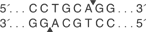
\includegraphics[scale=.5]{Sbf-I-cutsite_1_v1_000015}} }
\newglossaryentry{SbfI}{name=SbfI, description={restriction enzyme with the recognition sequence CCTGCA$\downarrow$GG} }
\newglossaryentry{XhoI}{name=XhoI, description={restriction enzyme with the recognition sequence C$\downarrow$TCGAG} }
\newglossaryentry{heterochromatin}{name=heterochromatin, description={Chromatin that remains in a highly condensed state throughout the cell cycle}}
\newglossaryentry{contig}{name=contig, description={longer consensus sequence derived from assembling smaller overlapping sequence reads}}
\newglossaryentry{linked RAD tag site}{name=linked RAD tag site, description={position in the reference sequence with at least one \gls{concordant} read pair on each side of a putative restriction site and the SE reads overlapping each other as expected from the restriction enzyme}}
\newglossaryentry{proper pair}{name=proper pair, description={read pair from illumina paired-end sequencing that got mapped to a reference in the correct orientation within a maximum expected distance from each other that is determined by the fragment size selection during the sequencing library preparation. Also called a \gls{concordant}ly mapping pair}}
\newglossaryentry{kmer}{name=kmer, description={subsequence with a specified length (k) of a longer sequence}}
\newglossaryentry{e-value}{name=Expect (E) value, description={The Expect value (E) is a parameter that describes the number of hits one can "expect" to see by chance when searching a database of a particular size}}
\newglossaryentry{read}{name=read, description={any sequence that comes out of the sequencer}}
\newglossaryentry{edit distance}{name=edit distance, description={minimum number of operations (one symbol insertion, deletion or substitution) required to change one string of symbols into another. Also known as \emph{Levenshtein distance}}}
\newglossaryentry{Ct}{name={C$_{t}$}, description={PCR cycle when a certain fluorescent threshold is reached}}
\newglossaryentry{mqs}{name={mapping quality score}, description={The mapping quality score \emph{Q} is the Phred transformation of the estimate of the probability \emph{p} that the reported mapping position does not correspond to the read's true point of origin: $Q = -10 \log_{10} p$. The way \emph{p} is estimated is different for each mapping programme, but in any case a mapping quality score \emph{Q} of 3 roughly corresponds to a mis-mapping probability \emph{p} of 0.5, i. e. the read has an estimated 50\% chance to have derived from a location other than the one reported}}
\newglossaryentry{discordant}{name=discordant, description={A read pair is called discordant if it aligns without the expected relative mate orientation (here: forward--reverse or reverse--forward) or outside the expected range of distances between mates. Note that \texttt{bowtie2} only calls discordant read pair mappings if both reads map \emph{uniquely}. Here, I am NOT adopting this requirement}}
\newglossaryentry{concordant}{name=concordant, description={A read pair is called concordant if it aligns with the expected relative mate orientation (here: forward--reverse or reverse--forward) and within the expected range of distances between mates. This is also called a \gls{proper pair}. The complement of \gls{discordant}}}
\newglossaryentry{Levenshtein distance}{name=Levenshtein distance, description={The Levenshtein distance is equal to the minimum number of operations (edits) required to transform one string into another. The allowed operations are single character insertions, deletions and substitutions. This is also known as edit distance.}}
\newglossaryentry{all pairs}{name={all pairs}, description={all the pairs of sequences below a given Levenshtein distance are identified during the graph construction phase}}
\newglossaryentry{transitive clusters}{name=transitive clusters, description={Two read clusters are merged if the distance of any pair of reads between the clusters is below threshold. After merging, the newly created cluster can contain read pairs with distance above the clustering threshold}}
\newglossaryentry{graph}{name=graph, description={A network of connected sequences. Two sequences are directly connected if they match with distance below a threshold. The distance is a measure of the strength of connection, aka "edge weight". Graphs can be stored as a list of pairs of sequences, with an optional edge weight. All graphs here should be "undirected cyclic graphs"}}
\newglossaryentry{Nmer}{name=\emph{N}mer, description={synonymous to kmer, unit, word; a subsequence of size \emph{N} that is overlapping or contiguous with the next subsequence of size \emph{N} and stored in a dictionnary (aka hash) for fast lookup}}
\newglossaryentry{population allele frequency}{name=population allele frequency, description={The population allele frequency is the (unknown) frequency of the allele in the entire population}}
\newglossaryentry{sample allele frequency}{name=sample allele frequency, description={The sample allele frequency is the frequency of the allele among the individuals in a specific sample}}
\newglossaryentry{connected component}{name=connected component, description={All nodes (here sequence reads) after all--pairs search (and before clustering!) that are directly connected by an edge or indirectly connected via several nodes belong to the same connected component} }

%----------------
% Acronyms
%----------------
\newacronym{snp}{SNP}{single nucleotide polymorphism}
\newacronym{rad}{RAD}{Restriction Site associated DNA}
\newacronym{pe}{PE}{paired-end}
\newacronym{se}{SE}{single-end}
\newacronym{bp}{bp}{base pair}
\newacronym{Mbp}{Mbp}{mega base pairs}
\newacronym{Gbp}{Gbp}{giga base pairs}
\newacronym{indel}{indel}{small sequence insertion or deletion polymorphism}
\newacronym{SAM}{SAM}{Sequence Alignment/Map format}
\newacronym{EST}{EST}{expressed sequence tag}
\newacronym{ddRAD}{ddRAD}{double digest RAD}
\newacronym{ML}{ML}{maximum likelihood}
\newacronym{SFS}{SFS}{site frequency spectrum}
\newacronym{HWE}{HWE}{Hardy Weinberg equilibrium}
\newacronym{CI}{CI}{confidence interval}
\newacronym{EM}{EM}{Expectation Maximisation}
\newacronym{DEM}{DEM}{digital elevation model}
%\usepackage[toc]{glossaries}
%\renewcommand*{\glstextformat}[1]{\textsf{#1}}
%
%\newglossaryentry{fragment}{name=fragment, description={not a PCR duplicate}}
%
%\newacronym{snp}{SNP}{single nucleotide polymorphism}

%% ******************************** SVG *************************************
%\newcommand{\executeiffilenewer}[3]{%
%	\ifnum\pdfstrcmp{\pdffilemoddate{#1}}%
%	{\pdffilemoddate{#2}}>0%
%	{\immediate\write18{#3}}\fi%
%}
%\newcommand{\includesvg}[1]{%
%	\executeiffilenewer{#1.svg}{#1.pdf}%
%	{./inkscape -z -D -f #1.svg %
%	--export-pdf=#1.pdf --export-latex}%
%	\import{./Figs/Inkscape_Graphics}{#1.pdf_tex}%
%}



%******************************** Glossary *********************************************
% *** \usepackage[toc,acronym]{glossaries}
% suppress page number list in glossary:
%\usepackage[nonumberlist]{glossaries}

%
% -- put the following code into a .latexmkrc file in the directory from where you run Latexmk --
%
%# add glossary generation to LATEXMK routine
%# ==========================================
%# taken from:
%# http://tex.stackexchange.com/questions/1226/how-to-make-latexmk-use-makeglossaries
%
%add_cus_dep('glo', 'gls', 0, 'run_makeglossaries');
%add_cus_dep('acn', 'acr', 0, 'run_makeglossaries');
%
%sub run_makeglossaries {
%  if ( $silent ) {
%    system "makeglossaries -q $_[0]";
%  }
%  else {
%    system "makeglossaries $_[0]";
%  };
%}
%
%push @generated_exts, 'glo', 'gls', 'glg';
%push @generated_exts, 'acn', 'acr', 'alg';
%$clean_ext .= ' %R.ist %R.xdy';

\makeglossaries

\renewcommand*{\glstextformat}[1]{\textsf{#1}}
%\renewcommand*{\glshyperlink}[1]{\textsf{#1}}

%--------------
% Glossary
%--------------
\newglossaryentry{fragment}{name=fragment, description={not a PCR duplicate. With paired reads from standard RAD (i. e. including random shearing of restriction fragments) typically identified by having different PE read sequences or different insert sizes after read mapping against a reference}}
\newglossaryentry{RAD tag}{name=RAD tag, description={genetic marker from RAD sequencing; the sequence up or downstream of a restriction site}}
\newglossaryentry{barcode}{name=barcode, description={short DNA sequence incorporated into adapter oligonucleotides that becomes part of the sequence read. Barcodes are used in order to be able to pool the DNA of different individuals, populations, treatments, etc. into one library that can be sequenced on one lane of an illumina flow cell}}
\newglossaryentry{index}{name=index, description={similar to barcode and serves the same purpose; generally incorporated into the centre of the adapter so that special sequencing run for the index is required} }
%\newglossaryentry{SbfI}{name=SbfI, description={restriction enzyme with the recognition sequence 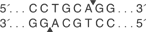
\includegraphics[scale=.5]{Sbf-I-cutsite_1_v1_000015}} }
\newglossaryentry{SbfI}{name=SbfI, description={restriction enzyme with the recognition sequence CCTGCA$\downarrow$GG} }
\newglossaryentry{XhoI}{name=XhoI, description={restriction enzyme with the recognition sequence C$\downarrow$TCGAG} }
\newglossaryentry{heterochromatin}{name=heterochromatin, description={Chromatin that remains in a highly condensed state throughout the cell cycle}}
\newglossaryentry{contig}{name=contig, description={longer consensus sequence derived from assembling smaller overlapping sequence reads}}
\newglossaryentry{linked RAD tag site}{name=linked RAD tag site, description={position in the reference sequence with at least one \gls{concordant} read pair on each side of a putative restriction site and the SE reads overlapping each other as expected from the restriction enzyme}}
\newglossaryentry{proper pair}{name=proper pair, description={read pair from illumina paired-end sequencing that got mapped to a reference in the correct orientation within a maximum expected distance from each other that is determined by the fragment size selection during the sequencing library preparation. Also called a \gls{concordant}ly mapping pair}}
\newglossaryentry{kmer}{name=kmer, description={subsequence with a specified length (k) of a longer sequence}}
\newglossaryentry{e-value}{name=Expect (E) value, description={The Expect value (E) is a parameter that describes the number of hits one can "expect" to see by chance when searching a database of a particular size}}
\newglossaryentry{read}{name=read, description={any sequence that comes out of the sequencer}}
\newglossaryentry{edit distance}{name=edit distance, description={minimum number of operations (one symbol insertion, deletion or substitution) required to change one string of symbols into another. Also known as \emph{Levenshtein distance}}}
\newglossaryentry{Ct}{name={C$_{t}$}, description={PCR cycle when a certain fluorescent threshold is reached}}
\newglossaryentry{mqs}{name={mapping quality score}, description={The mapping quality score \emph{Q} is the Phred transformation of the estimate of the probability \emph{p} that the reported mapping position does not correspond to the read's true point of origin: $Q = -10 \log_{10} p$. The way \emph{p} is estimated is different for each mapping programme, but in any case a mapping quality score \emph{Q} of 3 roughly corresponds to a mis-mapping probability \emph{p} of 0.5, i. e. the read has an estimated 50\% chance to have derived from a location other than the one reported}}
\newglossaryentry{discordant}{name=discordant, description={A read pair is called discordant if it aligns without the expected relative mate orientation (here: forward--reverse or reverse--forward) or outside the expected range of distances between mates. Note that \texttt{bowtie2} only calls discordant read pair mappings if both reads map \emph{uniquely}. Here, I am NOT adopting this requirement}}
\newglossaryentry{concordant}{name=concordant, description={A read pair is called concordant if it aligns with the expected relative mate orientation (here: forward--reverse or reverse--forward) and within the expected range of distances between mates. This is also called a \gls{proper pair}. The complement of \gls{discordant}}}
\newglossaryentry{Levenshtein distance}{name=Levenshtein distance, description={The Levenshtein distance is equal to the minimum number of operations (edits) required to transform one string into another. The allowed operations are single character insertions, deletions and substitutions. This is also known as edit distance.}}
\newglossaryentry{all pairs}{name={all pairs}, description={all the pairs of sequences below a given Levenshtein distance are identified during the graph construction phase}}
\newglossaryentry{transitive clusters}{name=transitive clusters, description={Two read clusters are merged if the distance of any pair of reads between the clusters is below threshold. After merging, the newly created cluster can contain read pairs with distance above the clustering threshold}}
\newglossaryentry{graph}{name=graph, description={A network of connected sequences. Two sequences are directly connected if they match with distance below a threshold. The distance is a measure of the strength of connection, aka "edge weight". Graphs can be stored as a list of pairs of sequences, with an optional edge weight. All graphs here should be "undirected cyclic graphs"}}
\newglossaryentry{Nmer}{name=\emph{N}mer, description={synonymous to kmer, unit, word; a subsequence of size \emph{N} that is overlapping or contiguous with the next subsequence of size \emph{N} and stored in a dictionnary (aka hash) for fast lookup}}
\newglossaryentry{population allele frequency}{name=population allele frequency, description={The population allele frequency is the (unknown) frequency of the allele in the entire population}}
\newglossaryentry{sample allele frequency}{name=sample allele frequency, description={The sample allele frequency is the frequency of the allele among the individuals in a specific sample}}
\newglossaryentry{connected component}{name=connected component, description={All nodes (here sequence reads) after all--pairs search (and before clustering!) that are directly connected by an edge or indirectly connected via several nodes belong to the same connected component} }

%----------------
% Acronyms
%----------------
\newacronym{snp}{SNP}{single nucleotide polymorphism}
\newacronym{rad}{RAD}{Restriction Site associated DNA}
\newacronym{pe}{PE}{paired-end}
\newacronym{se}{SE}{single-end}
\newacronym{bp}{bp}{base pair}
\newacronym{Mbp}{Mbp}{mega base pairs}
\newacronym{Gbp}{Gbp}{giga base pairs}
\newacronym{indel}{indel}{small sequence insertion or deletion polymorphism}
\newacronym{SAM}{SAM}{Sequence Alignment/Map format}
\newacronym{EST}{EST}{expressed sequence tag}
\newacronym{ddRAD}{ddRAD}{double digest RAD}
\newacronym{ML}{ML}{maximum likelihood}
\newacronym{SFS}{SFS}{site frequency spectrum}
\newacronym{HWE}{HWE}{Hardy Weinberg equilibrium}
\newacronym{CI}{CI}{confidence interval}
\newacronym{EM}{EM}{Expectation Maximisation}
\newacronym{DEM}{DEM}{digital elevation model}

%%%%%% -- KNITR SETUP -- %%%%%%%%%%

%%%%%%%%%%%%%%%%%%%%%%%%%%
\IfFileExists{upquote.sty}{\usepackage{upquote}}{}
\begin{document}

\tableofcontents

\listoffigures

\listof{cmd}{List of commands}

\printglossaries

\chapter{Testing incomplete digestion}

% **************************** Define Graphics Path **************************
%% Note, every path needs to end with a "/" !!!
\ifpdf
    \graphicspath{
    {./Figs/Raster/}
    {./Figs/PDF/}
    {./Figs/}
    {../Data_analysis/reference-mapping/figure/}
    }
\else
    \graphicspath{ 
    {./Figs/Vector/}
    {./Figs/}
%    {/Users/Claudius/Documents/PhD/THESIS/kks32/LaTeX/3_Chapter/Figs}
    }
\fi


% ************************************************************************************

%\epigraph{Nothing in biology makes sense, except in the light of evolution}{Theodosius Dobzhansky}
%
%\epigraph{\dots it occurred to me to ask the question, Why do some die and some live? And the answer was clearly, that on the whole the best fitted live. [\dots] Then it suddenly flashed upon me that this self-acting process would necessarily improve the race, because in every generation the inferior would inevitably be killed off and the superior would remain-that is, the fittest would survive \dots}{Alfred Russel Wallace}

\epigraph{
Bonzai: Are you as successful as you would like to be?

Zappa: I would say that the basic characteristic of my life is failure. 
If there is one thing that I excel at, it's failure -- I manage to fail at 100 percent of the things that I do. 
Since most of the things that I set out to do are theoretically impossible, it's very easy to fail. 
I've learned to live with it. 
In terms of machinery and personnel, there never seems to be enough to get things done exactly right.
}{interview with Frank Zappa, 1985}

% ------------------------------------------------------------------------------------------------

% ------------------------------------------------------------------------------------------------

% --------------------------------
\section{Introduction}
% --------------------------------
The initial goal was to do a hybrid zone analysis and a QTL mapping study with a genetic marker technique that would allow the reliable scoring of genotypes at 1000$+$ loci in the genome of the grasshoppers at relatively low cost. The \gls{rad} marker technique, first described by \cite{Baird2008}, seemed to fulfil that promise.

%% ------------------------------------
\subsection{Why use RAD?}
%% ------------------------------------
\gls{rad}, aka RADseq, is the high-throughput sequencing of restriction fragment ends (figure \ref{RAD_protocol_overview}). It requires no prior genome sequence information. Only genome size and GC content are required to estimate the required number of \glspl{read} for a certain target coverage. 
RADseq can yield co-dominant \gls{snp} markers in \glspl{RAD tag}, dominant presence/absence markers when the restriction site sequence is polymorphic or short indel polymorphisms when the clustering algorithm allows for them. Additionally, when doing \gls{pe} sequencing, a \gls{pe} contig can be assembled for a given \gls{RAD tag} (figure \ref{RAD_protocol_overview}).
Given enough coverage and when using adapters with barcode sequences, individual genotypes can be scored which is required for hybrid zone analysis (especially genomic clines analysis) as well as QTL mapping. 

Since the original version of \gls{rad} sequences tags around every restriction site (figure \ref{RAD_protocol_overview}), it allows for only limited complexity reduction. Further complexity reduction can be achieved by skipping the step of shearing the restriction fragments and instead size selecting a range of restriction fragments that have the right size for the sequencing platform. Further fine tuning of fragment number can be achieved when digesting DNA with two enzymes, so-called double-digest \gls{rad} (figure \ref{ddRAD_protocol_overview}) \citep{Peterson2012}.
% ---- add glossary entrywithout generating text ----
\glsadd[]{barcode} % allows to use \glshyperlink in captions

\begin{figure}
\centering
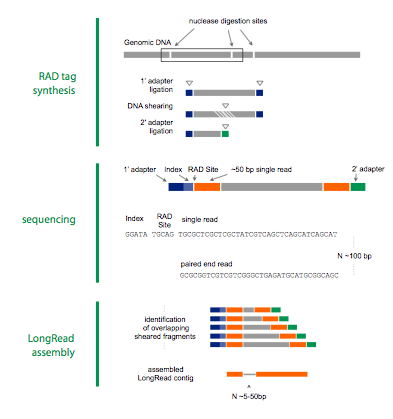
\includegraphics[width=.7\textwidth]{RADprotocolOverview}
\caption[Overview of the RAD marker technique.]{Overview of the \gls{rad} marker technique. (1) One restriction enzyme is used to digest genomic DNA. The first illumina adapter (P1), containing a different \glshyperlink[\textsf{barcode}]{barcode} (here called \gls{index}) sequence for each individual, is then ligated to the restriction fragments. The restriction fragments are then sheared, usually by high-frequency sonication, into a fragment size range that is suitable for illumina sequencing, which is selected on an agarose gel. After ligation of the second illumina adapter (P2), fragments with at least one P1 adapter are enriched by selective PCR. (2) The \gls{se} reads start with a barcode sequence, followed by the remainder of the restriction site. Only relatively short sequences (tags) are generated from the ends of the fragments. (3) Due to random shearing of restriction fragments, the \gls{pe} reads start at variable genomic distance from the restriction site (unless they are PCR duplicates) and thus can be assembled into short \gls{pe} contigs, depending on the size range selected on the gel. Taken from \cite{Atwood2011}. }
\label{RAD_protocol_overview}
\end{figure}

\begin{figure}
%
\includegraphics[width=\textwidth]{/Users/Claudius/Documents/PhD/sRAD/RAD_sketches/RAD_sketches}\\
%\includegraphics[width=\textwidth]{/Users/Claudius/Documents/PhD/sRAD/RAD_sketches/RAD_sketches_1}\\
\def\svgwidth{.9\textwidth}
\subimport{./Figs/Inkscape_Graphics/}{ddRAD_overview_1.pdf_tex}\\ 
\def\svgwidth{\textwidth}
\subimport{./Figs/Inkscape_Graphics/}{ddRAD_overview_2.pdf_tex}\\
\def\svgwidth{.9\textwidth}
\subimport{./Figs/Inkscape_Graphics/}{ddRAD_overview_3.pdf_tex}\\
\def\svgwidth{.9\textwidth}
\subimport{./Figs/Inkscape_Graphics/}{ddRAD_overview_4.pdf_tex}\\
\def\svgwidth{.9\textwidth}
\subimport{./Figs/Inkscape_Graphics/}{ddRAD_overview_5.pdf_tex}
\caption[Double-digest RAD protocol overview.]{Double-digest RAD protocol overview.}
\label{ddRAD_protocol_overview}
\end{figure}

\begin{figure}[t]
\ContinuedFloat
\caption[]{Genomic DNA is first digested by two different restriction enzymes (red and green). Illumina adapters (P1 and P2) are then ligated to the restriction fragments. The P2 adapter is a so-called divergent-Y adapter that, if anything, only contains the reverse-complement of the backward PCR primer binding site needed during the selective PCR step (see figure \ref{adapter_outline}). Restriction fragments are then size-selected on a gel. Here, in contrast to the standard RAD protocol (see fig. \ref{RAD_protocol_overview}), gel size selection selects which markers get into the final sequencing library. The selective PCR step enriches the library for fragments with at least one P1 adapter ligated to it. Bridge-amplification on the illumina flow cell requires a P1 and a P2 adapter. Illumina paired-end sequencing results in two RAD tags per fragment that can be assembled and used for SNP and indel calling.}
\end{figure}


%% ------------------------------------
\subsection{The Problem}
%% ------------------------------------

A standard RAD library with the restriction enzyme \gls{SbfI} was prepared according to the protocol of Paul Etter, (University of Oregon, \citealt{Baird2008}). The RAD library contained DNA from 36 grasshoppers sampled from the two distal populations ("Aunat" and "Greixer") of a transect through the \textit{Chorthippus parallelus / erythropus} hybrid zone in the Pyrenees between France and Spain. The RAD library was sequenced on an illumina GAIIx and the resulting reads assembled with the programme suite \texttt{stacks} \citep{Catchen2011}.

Figure \ref{Big_Data:freq_dist_of_genotype_calls} shows the frequency distribution of loci -- reconstructed by \texttt{stacks} version 0.998 -- over the number of individuals that have a genotype called for that locus. \texttt{Stacks} was run with a minimum allele coverage of 3 per individual and a maximum number of mismatches between alleles of 2 for merging alleles into loci within individuals as well as assembling a catalog of loci for the whole sample of 36 grasshoppers (further details can be looked up on the \href{http://creskolab.uoregon.edu/stacks/param_tut.php}{\texttt{stacks}} home page). About 50\% of the 379,720 unfiltered reconstructed loci have only a genotype call in one or two of the 36 individuals. About 170,000 RAD markers were expected from this library (see section \ref{ch:RAD_marker_number}) assuming a genome size of 12 giga \glspl{bp} (see section \ref{ch:Genome_size}).

%\begin{figure}
%\centering
%<<freq dist of genotype calls Big Data, echo=FALSE, out.width='.9\\linewidth', cache=TRUE>>=
%@
%\caption{Frequency distribution of loci, reconstructed by \texttt{stacks} (i. e. so-called "catalog stacks"), over the number of individuals in which they have a genotype call.}
%\label{Big_Data:freq_dist_of_genotype_calls}
%\end{figure}

Figure \ref{ddRAD:freq_dist_of_genotype_calls} shows the frequency distribution of reconstructed loci over the number of individuals for which they have a genotype called for the data of an \gls{SbfI}$+$\gls{XhoI} double-digest RAD library. The \gls{se} and \gls{pe} \glspl{RAD tag} have been merged before the assembly with \texttt{stacks}. \texttt{Stacks} was run with a minimum allele depth of 3 and maximum mismatch distance of 6 for merging alleles into read stacks within individuals as well as assembling a catalog stack from the individual stacks of all 36 grasshoppers (plus 2 technical replicates). Of the 156,532 loci (i. e. catalog stacks) that \texttt{stacks} had assembled, 51\% can only be found in one individual and only 3.5\% can be found in 20 or more individuals. Around 16,000 RAD markers were expected from this double-digest library (see equation \ref{eq:exp_number_ddRAD_loci} in chapter \ref{ch:RAD_marker_number}).

%\begin{figure}
%\centering
%<<freq dist of genotype calls SbfI-XhoI, echo=FALSE, out.width='.9\\linewidth', cache=TRUE>>=
%@
%\caption{Frequency distribution of catalog tags over the number of individuals in which they have a genotype call.}
%\label{ddRAD:freq_dist_of_genotype_calls}
%\end{figure}

\begin{figure}
\centering
\begin{subfigure}[t]{.495\textwidth}
\begin{knitrout}
\definecolor{shadecolor}{rgb}{0.969, 0.969, 0.969}\color{fgcolor}

{\centering \includegraphics[width=.9\linewidth]{figure/freq_dist_of_genotype_calls_Big_Data-1} 

}



\end{knitrout}
\caption{}
\label{Big_Data:freq_dist_of_genotype_calls}
\end{subfigure}
\hfill
\begin{subfigure}[t]{.495\textwidth}
\begin{knitrout}
\definecolor{shadecolor}{rgb}{0.969, 0.969, 0.969}\color{fgcolor}

{\centering \includegraphics[width=.9\linewidth]{figure/freq_dist_of_genotype_calls_SbfI-XhoI-1} 

}



\end{knitrout}
\caption{}
\label{ddRAD:freq_dist_of_genotype_calls}
\end{subfigure}
\caption{Frequency distribution of loci, reconstructed by \texttt{stacks} (i. e. so-called "catalog stacks"), over the number of individuals in which they have a genotype call.}
\label{freq_dist_of_genotype_calls}
\end{figure}


In the standard RAD data set, there are 5,014 SE reads and 25,268 PE reads that apparently contain SbfI recognition sites within them (30,282 in total)\footnote{counted with \texttt{grep -c}}. I searched in 88,734,712 quality filtered reads altogether. That is, 0.034\% of quality filtered reads contain an SbfI recognition site. Figure \ref{SbfI_frequency_dist_per_ind} shows the frequency distributions of SbfI sites in SE and PE reads for all 36 individuals separately. Obviously, if SbfI restriction and following P1 adapter ligation were 100\% efficient, there should be no SbfI recognition sequences in either SE or PE reads. 

\begin{figure}[htb]
\centering
\begin{knitrout}
\definecolor{shadecolor}{rgb}{0.969, 0.969, 0.969}\color{fgcolor}

{\centering 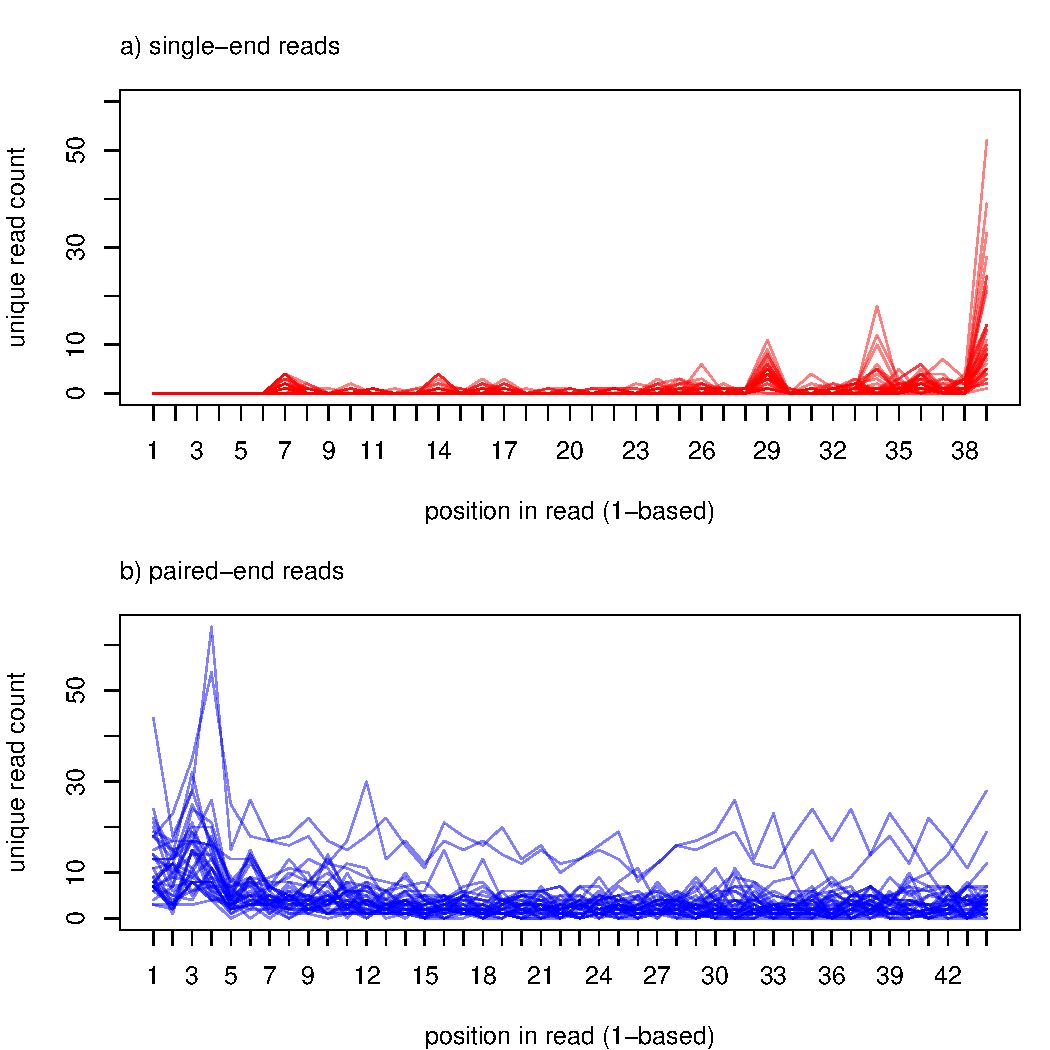
\includegraphics[width=.8\linewidth]{figure/SbfI_frequency_dist__per_ind_-1} 

}



\end{knitrout}
\caption{SbfI site frequency spectrum across (a) SE and (b) PE reads for each of the 36 individuals}
\label{SbfI_frequency_dist_per_ind}
\end{figure}


Could this pattern be an indication that SbfI restriction during the library preparation was incomplete? If so, could there be systematic variation between individuals  in the completeness of SbfI restriction that could lead to many loci only being detected in a few individuals as shown in figure \ref{freq_dist_of_genotype_calls}?
Incomplete digestion for a specific SbfI site could in principle be tested with a PCR (or more quantitatively with qPCR) across this site before and after digestion \citep{Luca2011}. However, no close reference sequence is available for PCR primer design\footnote{as of April 2014}. For a given \gls{RAD tag} from a standard RAD library, the PE reads can be used to assemble them into a \gls{contig} that could be long enough for primer design (see figure \ref{RAD_protocol_overview}).
Still, for PCR primer design, \emph{pairs} of PE \glspl{contig} need to be created. This requires some reference sequence to provide the information which \glspl{RAD tag} come from the same SbfI site in the genome.


%% ---------------------------------------------------
\section{Methods \& Results}
%% ---------------------------------------------------

I used the transcriptome of the desert locust \textit{Schistocerca gregaria} (\textit{Cyrtacanthacridinae}) \citep{Badisco2011} as a reference sequence. The transcriptome of another grasshopper -- \textit{Locusta migratoria} (\textit{Oedipodinae}) \citep{Kang2004} -- was also available, but \cite{Liu2008a} have shown that the family \textit{Cyrtacanthacridinae} is more closely related to \textit{Gomphocerinae} -- the family that \textit{Chorthippus parallelus} belongs to -- than the family \textit{Oedipodinae}.

I have mapped the standard RAD reads\footnote{informal name "Big Data"} of all 36 individuals against the \textit{Schistocerca} transcriptome with \texttt{stampy} \citep{Lunter2011} (see \vref{ch:read_mapping}). I merged all individual mapping output files into one big file with \texttt{samtools merge} and ran my custom script \texttt{find\_linked\_RADtags.pl} on it (further description in section \ref{ch:find_linked_RADtags}). That way, I extracted from all individuals all PE reads that belong to a \gls{linked RAD tag site} that was detected in as little as one individual.

In order to design PCR primers I need to assemble the paired-end reads from single-end reads that map to the same restriction site. The \texttt{find\_linked\_RADtags.pl} script required at least one \gls{proper pair} of reads mapping on either side of a restriction site to detect a contig from the transcriptome reference. It detected 77 \textit{Schistocerca} reference contigs with \glspl{linked RAD tag site}.

I used the programme \texttt{SSAKE} \citep{Warren2007} together with my wrapper script \texttt{SSAKEoptimiser.pl} for the de novo assembly of \gls{pe} contigs (see section \ref{ch:PE_read_assembly}). \texttt{SSAKEoptimiser.pl} finds the optimal \gls{kmer} length for each individual assembly, optimising for the length of the longest contig assembled. There are 64 \textit{Schistocerca} reference contigs with a RAD tag site for which at least one upstream and one downstream \texttt{SSAKE} contig could be assembled.

The \texttt{SSAKEoptimiser} output for each assembly generally contains several \glspl{contig} of similar length and with similar read counts. It is therefore not straightforward to pick those \texttt{SSAKE } contigs upstream and downstream of the restriction site that genuinely belong together, i. e. come from the same locus. For 20 \textit{Schistocerca} cDNA contigs I could assemble and confidently pick down and upstream \texttt{SSAKE} contigs for PCR primer design (see section \ref{ch:picking_right_contig}). 

I combined pairs of PE contigs by aligning them to their putative \textit{Schistocerca} reference contig and filled the gap between them with N's. I then used these 20 newly created \textit{C. parallelus} consensus sequences as a reference against which to map all standard SbfI-RAD reads. I would like to know how many of the 36 individuals get reads mapped to these \glspl{linked RAD tag site} and whether individuals have reads mapped to both \glspl{RAD tag} at an SbfI restriction site.

Among the 20 \emph{PE contig pair} reference sequences, there are 5 which:

\begin{itemize}
\item do not show very high or very low number of reads mapped
\item do not show large numbers of very divergent reads mostly containing \glspl{indel}
\item do not show other signs of repetitiveness, e. g. SE reads mapping to PE contigs instead of the \glspl{RAD tag}
\end{itemize}

One of these 5 reference sequences has only reads mapped from \textit{C. p. parallelus} (12 individuals) and none from \textit{C. p. erythropus}. This could be caused by a polymorphism in the restriction site sequence. For each individual, I counted the number of \glspl{fragment} mapped towards the remaining four reference sequences by taking only SE reads from \glspl{proper pair} and \texttt{uniq}-ing on insert size\footnote{i. e. collapsing multiple occurrences of the same insert size into one}. Figure \ref{fragments-mapped-per-ind} shows the distribution of these counts over all 36 individuals for the four \emph{PE contig pair} reference sequences.

\begin{figure}
\begin{knitrout}
\definecolor{shadecolor}{rgb}{0.969, 0.969, 0.969}\color{fgcolor}

{\centering 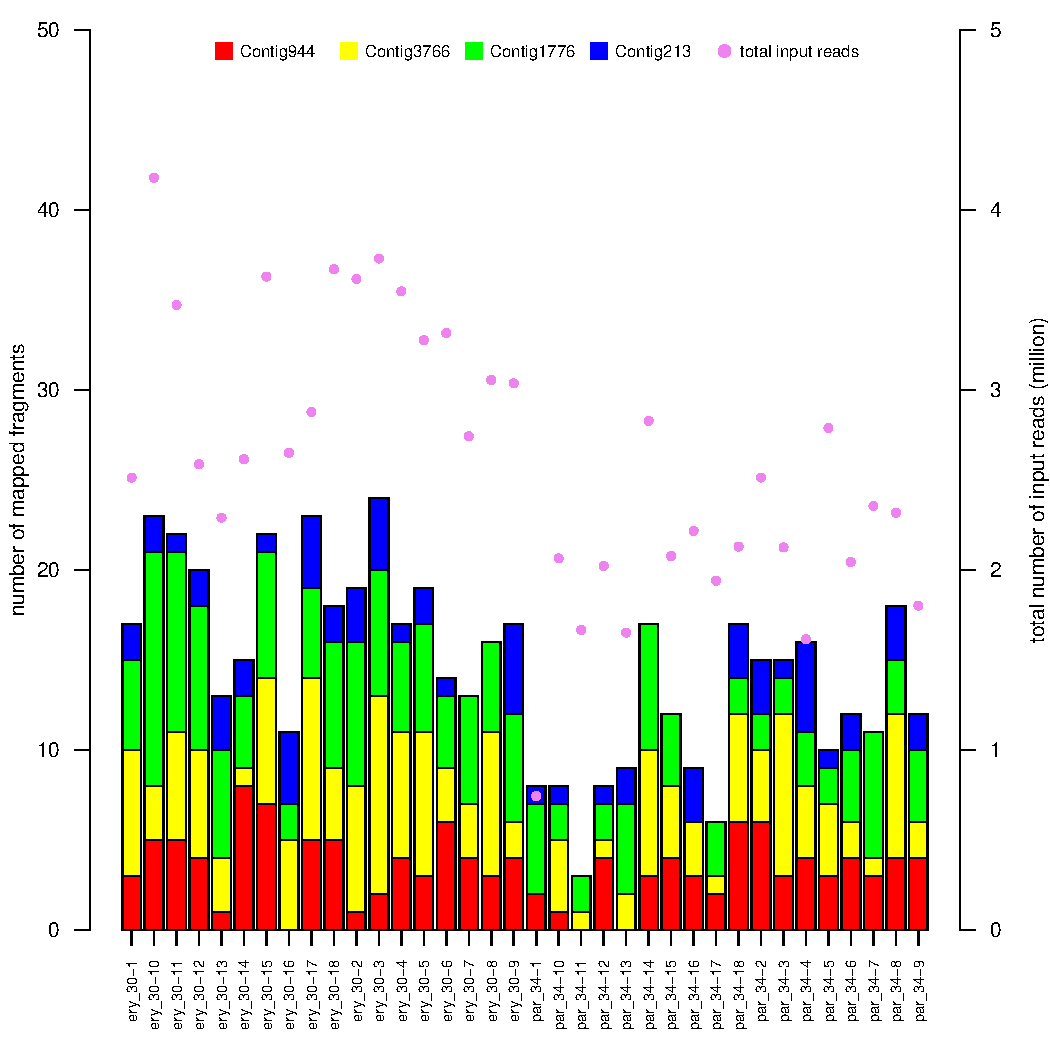
\includegraphics[width=\linewidth]{figure/fragments_mapped_per_ind-1} 

}



\end{knitrout}
\caption{Distribution of RAD \gls{fragment} numbers mapped to 4 \emph{PE contig pair} reference sequences.  
If two read pairs on a RAD site from an individual have the same insert size, they constitute only one fragment, i. e. one read pair is likely to be a PCR duplicate.}
\label{fragments-mapped-per-ind}
\end{figure}

Figure \ref{fragments-mapped-per-ind} indicates that none of the 4 loci is a good candidate to test possible variation in restriction enzyme digestion with PCR. The distribution of coverage at the 4 loci is rather even across the 36 individuals. Even though between individual variation in the completeness of digestion cannot be ruled out by this data yet, a different pattern would be expected if it was common. That is, more individuals would have no fragments mapping while others would have many. Given this data, incomplete digestion is now less likely to be the reason for the dominance of singleton loci in the \texttt{stacks} assembly (see figure \ref{freq_dist_of_genotype_calls}). The variation in coverage among individuals in figure \ref{fragments-mapped-per-ind} can largely be explained by variation in the number of input reads (figure \ref{frag_input_corr_fig}).

\begin{figure}
\begin{knitrout}
\definecolor{shadecolor}{rgb}{0.969, 0.969, 0.969}\color{fgcolor}

{\centering \includegraphics[width=.49\linewidth]{figure/fragments_input_reads_corr-1} 
\includegraphics[width=.49\linewidth]{figure/fragments_input_reads_corr-2} 

}



\end{knitrout}
\caption{Correlation of locus dropout (left) and fragment counts (right) with number of input reads. Left: Locus dropout is the number of loci (which are the same as in figure \ref{fragments-mapped-per-ind}) for which an individual had no \gls{fragment} mapped. Right: the sum of mapped \glspl{fragment} over the four loci for each individual versus the number of input reads for the read mapping.}
\label{frag_input_corr_fig}
\end{figure}

The \gls{fragment} count is generally not very high (see table \ref{mean_sd_fragNum_per_locus}), indicating that low unique template amount for sequencing prevented any individual from having many fragments mapped. I started the standard SbfI RAD library preparation with about 130 ng of DNA from each grasshopper. Assuming that the genome is 12 Gbp long (see section \ref{ch:Genome_size}), this would only correspond to 9,884 copies of the genome (equation \ref{eq:genome_copies}).

% latex table generated in R 3.1.2 by xtable 1.7-4 package
% Sun Apr 26 18:52:20 2015
\begin{table}[ht]
\centering
\caption{Mean and coefficient of variation of fragment counts for the 4 loci shown in figure \ref{fragments-mapped-per-ind}.} 
\label{mean_sd_fragNum_per_locus}
\begin{tabular}{rrr}
  \toprule
 & mean & CV \\ 
  \midrule
Contig944 & 3.5 & 0.5 \\ 
  Contig3766 & 4.5 & 0.6 \\ 
  Contig1776 & 4.8 & 0.5 \\ 
  Contig213 & 1.9 & 0.8 \\ 
   \bottomrule
\end{tabular}
\end{table}



\footnotesize
\begin{align}
\text{molar amount of template} &= \frac{\text{amount of DNA}}{\text{MW of bp} \times \text{genome size}} 
= \frac{130 \times 10^{-9}\text{g}}{660 \frac{\text{g}}{\text{mol} \times \text{bp}} \times 12 \times 10^{9} \text{bp}} \label{eq:genome_copies} \\
&= 1.26 \times 10^{-20} \text{mol} \nonumber \\[5pt]
%\end{align}
%\begin{align}
\text{number of template molecules} &= 1.26 \times 10^{-20} \text{mol} \times \text{Avogadro's number} \nonumber \\
&= 1.26 \times 10^{-20} \text{mol} \times 6.0221413 \times 10^{23} \nonumber \\
&= 9884 \nonumber
\end{align}
\normalsize

The problem of low \gls{fragment} count is unlikely to be alleviated much by creating more sequence reads from this library (figure \ref{PCRduplicates}).

\begin{figure}
\begin{center}
\includegraphics[scale=0.7]{PCR_duplicates}
\caption{The same library was sequenced on four different illumina GAIIx flow cell lanes with increased sequence template amount resulting in an increased read yield. However, this increased sequencing effort for the same RAD library generated an ever higher proportion of PCR duplicates.}
\label{PCRduplicates}
\end{center}
\end{figure}

Instead, the template amount from each individual for the selective PCR during the library preparation needs to be increased. One obvious way would be to increase the total DNA input from each individual, but that reduces the number of individuals that can be pooled during the library preparation since the capacity of spin columns and the agarose gel (for size selection) is then reached with fewer individuals. Another option could be to postpone the gel fragment size selection until after a selective PCR, thus increasing the template amount for the PCR.

I used qPCR to estimate the template amount that went into my selective PCR's! See \texttt{../sRAD/qPCR} and my RAD\_double\_dig\_protocol

\begin{itemize}
\item template amount estimation with qPCR
\item check RAD protocols
\item incomplete digestion or just genomic religation?
\end{itemize}

%% ---------------------------------------------------
\section{Supplementary Methods}
%% ---------------------------------------------------

%% ---------------------------------------------------
\subsection{Adapter sequences for SbfI$+$XhoI ddRAD}\label{ch:adapter_sequences}
%% ---------------------------------------------------

\begin{figure}[h]
\begin{Verbatim}[fontfamily=courier, fontsize=\relsize{-7}, commandchars=\\\{\}, frame=single, framesep=10pt, label=P1 and P2 adapters for ddRAD]
          {\footnotesize P1 adapter}                                        {\footnotesize insert}                                   {\footnotesize P2 adapter}
5'-\underline{AATGATACGGCGACCACCGA}GATCTACACTCTTTCCCTACACGA\colorbox{white}{CGCTCTTCCGATCT}xxxxx{\color{blue}TGC*A}     GGNNNNNNNNNNNC     P-{\color{red}TCGA}\colorbox{orange}{A-GATCGGAAGAGCG}GTTCAGCAGGAATGCCGAGACCG\rotatebox{30}{\textit{TAGAGCATA*C}-3'}
3'-TTACTATGCCGCTGGTGGCTCTAGATGTGAGAAAGGGATGTGCT\colorbox{orange}{GCGAGAAGGCTAGA}xxxxx-P    {\color{blue}ACGT}CCNNNNNNNNNNNG{\color{red}AGCT}       \colorbox{white}{T*CTAGCCTTCTCGC}CAAGTCGTCCTTACGGCTCTGGCTAG\underline{AGCATACGGCAGAAGACGAAC-5'}
\end{Verbatim}
\caption{Outline of P1 and P2 adapters for double-digest RAD. Underlined sequences are selective PCR primer sequences. An asterisk * stands for a phosphorothioate bond. A "P" stands for a phosphate group. Sequences in \textit{italics} are non-complementary (wavy). Sequences with an orange background are identical to each other. An "x" stands for a base in a barcode sequence.}
\label{adapter_outline} % note, label has to come after caption
\end{figure}


%% ---------------------------------------------------
\FloatBarrier
\subsection{Estimating genome wide GC content}\label{ch:gc}
%% ---------------------------------------------------

\begin{cmd}
\captionsetup{type=cmd} % this is necessary for the hyperlink to work, see manual for caption package, 6.5 about hyperref
\begin{Verbatim}[formatcom=\color{darkgray}, fontsize=\scriptsize]

$ for i in *fq_2.gz; do ( awk '(NR-2)%4==0' <(zcat $i) | perl -ne' $h{$_}=1;END{foreach $s (keys %h)
{$gc += $s =~ tr/GC/GC/;} print $gc/(51 * scalar keys %h), "\n";} ' )& done | 
perl -ne'$sum+=$_; END{print $sum/$., "\n";}'

0.4607
\end{Verbatim}
\caption[Determine GC content from standard RAD PE reads]{\small For each individual, this command takes the \glspl{pe} reads, uniques them and determines their overall GC content. Finally, the average of the individual GC contents is taken. Note the brute-force parallelisation by sending each iteration of the \texttt{for} loop into the background with \texttt{(\ldots )\&}.}
\label{cmd:GC_1}
\end{cmd}

Using the \gls{se} reads from the \gls{SbfI} RAD library (excluding the SbfI recognition sequence part) and command \ref{cmd:GC_2} I have determined the GC content of the \gls{se} reads: 49.5\%.

\begin{cmd}
\captionsetup{type=cmd} % this is necessary for the hyperlink to work, see manual for caption package, 6.5 about hyperref
\begin{Verbatim*}[formatcom=\color{darkgray}, fontsize=\scriptsize, numbers=left]
$ gc(){ awk '(NR-2)%4==0' | sed 's/^......//' |
perl -ne'$h{$_}=1;END{foreach $s (keys %h){$gc+=$s=~tr/GC/GC/;} print $gc/(40*scalar keys %h), "\n";}' ;}
$ export -f gc
$ mean(){ perl -ne'$sum+=$_; END{print $sum/$., "\n";}'; }
$ export -f mean
$ parallel -j 10 'zcat {} | gc' ::: *fq_1.gz | mean

0.4956
\end{Verbatim*}
\caption[Determine GC content of \gls{se} reads]{\small This command is a different version of command \ref{cmd:GC_1}. However, it is used here to determine the GC content of all \gls{se} reads from the standard \gls{SbfI} RAD library. It first creates and exports two functions, \texttt{gc} and \texttt{mean}, and then uses the programme \texttt{parallel} in order to parallelise the determination of GC content over 10 cores. After stripping barcode and the remainder of the restriction site, the reads are 40 base pairs long. Note, the space between \{ and \texttt{awk} (line 1) as well as \{ and \texttt{perl} (line 4) is required.}
\label{cmd:GC_2}
\end{cmd}

So, it seems that sequences close to \gls{SbfI} sites are more GC rich than further distant sequences. 

%% --------------------------------------------------------------------------------------------------------------------------
\FloatBarrier
\section{Genome size of \textit{Chorthippus parallelus}}\label{ch:Genome_size}
%% --------------------------------------------------------------------------------------------------------------------------

\textit{Chorthippus parallelus} has a chromosome complement of 2n = 16 + X. Males have one X-chromosomes, females have two. Table \ref{ta:genome_size_studies} shows four studies that provide genome size estimates for \textit{Chorthippus parallelus}. Note that all studies are measuring the DNA content of spermatids. However, none of the studies explicitly deal with the issue that half of their measurements are missing the contribution from the X chromosome. Table \ref{ta:genome_size_studies} mentions the country of origin of the grasshoppers used for genome size estimates. Note, however, that only \cite{Belda1991} provide sampling locations. For the rest it is assumed that individuals were sampled closed to the authors institutes. So two studies provide genome size estimates for \textit{C. parallelus parallelus} and two for \textit{C. parallelus erythropus}. The \textit{parallelus} subspecies seems to have a genome 2--4 giga \glspl{bp} larger than the one of subspecies \textit{erythropus}. Apart from possible systematic differences in methodology, this apparent difference in genome size could be real, since several studies have shown chromosomal differentiation between the two subspecies, in particular on the X chromosome: an active nucleolar organiser region (NOR) distally on the X in \textit{C. p. parallelus} but not in \textit{C. p. erythropus} \citep{Gosalvez1988}. This NOR on X lies in or near a distinctive distal C-band\footnote{\gls{heterochromatin} stained with Giemsa}. In addition, Pyrenean \textit{C. p. erythropus} also show an interstitial C-band on X that does not occur in pure \textit{C. p. parallelus} \citep{Bella2007}. Further chromosomal differences are listed in table 1 of \cite{Ferris1993}.

\ctable[
width=\textwidth,
doinside={ \relsize{-1.5} \setlength{\tabcolsep}{3pt} },
caption=Studies that provide genome size estimates for \textit{Chorthippus parallelus},
cap=Genome size estimates,
label=ta:genome_size_studies
]
{l c >{\raggedleft}p{.6cm}@{.}l >{\centering}p{2.5cm} l X}
{
\tnote[a]{\scriptsize see their table 3}
\tnote[b]{\scriptsize 5 individuals}
\tnote[c]{\scriptsize assuming 6.4 on relative scale corresponds to C-value of 5.5 pg}
\tnote[d]{\scriptsize see their table 2}
\tnote[e]{\scriptsize \textit{C. longicornis} syn. of \textit{C. parallelus}}
\tnote[f]{\scriptsize 3 individuals}
\tnote[g]{\scriptsize 3 individuals}
}
{
\toprule
\multirow{2}{*}{\textbf{study}} & \multirow{2}{1cm}{\textbf{sample source}}  & \multicolumn{2}{c}{\textbf{C-value}} & \multirow{2}{*}{\textbf{Method}} & \multirow{2}{*}{\textbf{tissue type}} & \multirow{2}{*}{\textbf{standard species}} \\
                                      &                                                              & \multicolumn{2}{c}{ [$10^{-12}$g]} &                                &                                                 &                                                           \\
\midrule
\cite{John1966}\tmark[a] & UK & 12&37 ($\pm$ 0.75)\tmark[b] & Feulgen staining, microdensitometry & spermatid & \textit{Locusta migratoria}\tmark[c] \\[0.7cm]
\cite{Wilmore1975}\tmark[d] & UK & 13&36 ($\pm$ 0.04) & Feulgen staining, microdensitometry & spermatid & mouse spermatid \\[0.7cm]
\cite{Gosalvez1980}\tmark[e] & Spain & 8&58 ($\pm$ 0.47)\tmark[f]   & Feulgen staining, microdensitometry & spermatid & \textit{Allium cepa}, root tissue \\[0.7cm]
\cite{Belda1991} & Spain & 10&73 ($\pm$ 0.97)\tmark[g]  & Feulgen staining, microdensitometry & spermatid & chick erythrocytes \\
\bottomrule
}

\cite{Gosalvez1988} showed that all the heterochromatin present in both subspecies is particularly rich in GC DNA base pairs.


%\begin{table}
%\caption{Studies that provide genome size estimates for \textit{Chorthippus parallelus}}
%\label{ta:genome_size}
%\centering
%\small
%\resizebox{\textwidth}{!}{
%\begin{tabular}[h]{c c >{\raggedleft}p{.6cm}@{.}l >{\centering}p{3cm} c c}
%\toprule
%\multirow{2}{*}{\textbf{study}} & \multirow{2}{1cm}{\textbf{sample source}}  & \multicolumn{2}{c}{\textbf{C-value}} & \multirow{2}{*}{\textbf{Method}} & \multirow{2}{*}{\textbf{tissue type}} & \multirow{2}{*}{\textbf{standard species}} \\
%                                      &                                                              & \multicolumn{2}{c}{ [$10^{-12}$g]} &                                &                                                 &                                                           \\
%\midrule
%\cite{John1966} & UK & 12&37 $\pm$ 0.75 & Feulgen staining, microdensitometry & spermatid & \textit{Locusta migratoria}\\[0.7cm]
%\cite{Wilmore1975} & UK & 13&36  & Feulgen staining, microdensitometry & spermatid & mouse spermatid \\[0.7cm]
%\cite{Gosalvez1980} & Spain & 8&58   & Feulgen staining, microdensitometry & spermatid & \textit{Allium cepa}, root tissue \\[0.7cm]
%\cite{Belda1991} & Spain & 10&73  & Feulgen staining, microdensitometry & spermatid & chick erythrocytes \\
%\bottomrule
%\end{tabular}
%}
%\end{table}


%% --------------------------------------------------------------------------------------------------------------------------
\FloatBarrier
\subsection{Expected RAD marker number}\label{ch:RAD_marker_number}
%% --------------------------------------------------------------------------------------------------------------------------

Using PE reads from the standard RAD library -- uniqued  per individual -- as a proxy for the whole genome, I estimate the GC content of the \textit{Chorthippus parallelus} genome to be around 46\% (\ref{ch:gc}). However, \cite{Wilmore1975} have determined the GC content of the \textit{C. p. parallelus} genome from thermal dissociation profiles (41.2\%) and sedimentation in CsCl and Cs$_{2}$SO$_{4}$ density gradients (41.7\% and 42.0\%)\footnote{see their table 1}. I think that \gls{pe} reads from SbfI standard RAD are still a biased sample towards GC rich regions of the genome due to the GC rich \gls{SbfI} recognition sequence. 
Assuming a genome size of 12 giga base pairs, the expected number of RAD tag loci from a standard RAD library with \gls{SbfI} in the grasshopper genome is $\sim$170,000 (equation \ref{eq:exp_num_standard_RAD_loci}). 

\scriptsize
\begin{align}
\text{expected number of \glspl{RAD tag}} &= \underbrace{12 \times 10^{9}}_{\text{genome size}} \times 
\underbrace{ \left( \frac{0.42}{2}\right)^{6} \times \left( \frac{(1-0.42)}{2} \right)^{2} }_{\text{SbfI site probability}} \times 
\underbrace{2}_{\text{tags per SbfI site}}
\label{eq:exp_num_standard_RAD_loci} \\[5pt] 
&= 173,110 \nonumber
\end{align}
\normalsize

The number (and identity) of markers in a double-digest RAD library depends very much on the size selection of restriction fragments. I selected fragments roughly between 300 and 800 \gls{bp} length. The P1 adapter is 63 bp long (excluding 4 bp overhang), the P2 adapter is 61 bp long (excluding 4 bp overhang). The \gls{SbfI} remainder after the cut is 6 \gls{bp} long and the \gls{XhoI} remainder is 5 \gls{bp} long. If \gls{XhoI} cuts a fragment at a distance less than about $300 - 63 - 61 -6 -5 = 165$ \gls{bp} away from the SbfI cut site, then this fragment would not be size selected because it would be shorter than the lower bound of size selection (in this example). The \gls{se} sequences (excluding the SbfI recognition sequence parts) have a mean GC content of 49.5\% (see command \ref{cmd:GC_2}). 
The following formula requires the GC content of sequences of length 168 \gls{bp} adjacent to SbfI sites. I will use the average of \gls{se} and \gls{pe} GC contents -- 48\% (see~chapter \ref{ch:gc}) -- for calculating the probability of an XhoI cut within the first 168bp after the SbfI restriction site. In the next 500 \gls{bp} then needs to be at least one \gls{XhoI} site to make the SbfI fragment a marker.
The expected number of RAD markers per genome with an SbfI-XhoI double-digest and a selected size range of 300--800bp is:


\scriptsize
%\begin{preview}
\begin{align} % use align instead of equation for multi-line long equations
\text{RAD markers per genome} &\simeq 12 \times 10^{9} 
	&&\text{(genome size in bp)}  \label{eq:exp_number_ddRAD_loci} \\[5pt]
&\times \left(\frac{0.42}{2}\right)^{6}\times \left(\frac{(1-0.42)}{2}\right)^{2} &&\text{(SbfI cut prob. per bp)} \notag \\[5pt]
&\times 2 
	&&\text{(each cut creates two potential RAD tags)} \notag \\[5pt]
&\times \left[1-\left(\frac{0.48}{2}\right)^{4} \times \left( \frac{(1-0.48)}{2}\right)^{2} \right]^{165} 
	&&\text{(prob. of no XhoI cut in the first 165 bp after SbfI site)} \notag \\[5pt]
&\times \left(1- \left[1-\left(\frac{0.46}{4}\right)^{2} \times \left( \frac{(1-0.46)}{4}\right)^{4} \right]^{500} \right) 
	&&\text{(prob. of at least one XhoI cut in the following 500bp)} \notag \\[5pt]
%&\quad \times \ 2 \tag{two markers per SbfI cut{\color{red}*}}  \\
&\simeq 16,000 \nonumber
\end{align}
%\end{preview}
\normalsize

I have created an Excel file called \texttt{ComplexityReduction.xls} that implements equation \ref{eq:exp_number_ddRAD_loci} and that allows easy modification of variables.


%% ---------------------------------------------------
\FloatBarrier
\subsection{Read mapping against reference sequence}\label{ch:read_mapping}
%% ---------------------------------------------------

49,351,479 \texttt{process\_radtags} quality filtered reads with ``-s 20'' (discard read if average quality score in the sliding window drops below 20). The 49 million reads had been quality filtered with \texttt{process\_radtags} from the \texttt{stacks} pipeline. The Big Data standard RAD reads used here (as in the previous section) were \texttt{process\_radtags} purified with a quality score threshold of 20 in a 20 bp sliding window. I used command \ref{cmd:sam_to_bam_via_awk_in_parallel} in order to extract all SAM records, where at least one read in a pair got mapped, with subsequent position sorting.

\begin{cmd}
\captionsetup{type=cmd} % this is necessary for the hyperlink to work, see manual for caption package, 6.5 about hyperref
\begin{Verbatim}[fontsize=\scriptsize, formatcom=\color{darkgray}]

for i in *sam.gz; \
do (samtools view -hS $i | gawk '/^\@/ || and($2, 4)==0 || and($2, 8)==0' | \
samtools view -uhS - | samtools sort - `basename $i .fq_1.sam.gz`) & done
\end{Verbatim}
\caption{Command line that uses \texttt{samtools} and \texttt{awk} to create position sorted bam files in parallel that only contain records of paired reads where at least one read of the pair got mapped (i. e. skipping records with flag 77 and 141). \scriptsize{Note the brackets around the command line and the skipping of ";" between "\&" and "done"}. }
\label{cmd:sam_to_bam_via_awk_in_parallel}
\end{cmd}

%% ---------------------------------------------------
\FloatBarrier
\subsection{\texttt{find\_linked\_RADtags.pl}}\label{ch:find_linked_RADtags}
%% ---------------------------------------------------

\gls{proper pair} (with a "properly mapped" pair on either side of the restriction site, see above)

Visually inspecting all contigs with \texttt{IGV} for whether they have read pairs mapped to both sides of one SbfI restriction site is very tedious and time consuming. So I wrote a script called \texttt{find\_linked\_RADtags.pl} which reports reference contigs where at least two read pairs map to opposite sites of an SbfI restriction site (or any cut site leaving a 4 bp overhang). This script also detects the contig shown in figure \ref{LC.1628.C1.Contig1776_standRAD}. With this script the detection of a reference contig requires one "properly" mapped read pair on either side of an SbfI restriction site. So SE as well as PE reads need to map on both sides of the restriction site. This is stringent and will obviously miss contigs with genuine SbfI RADtag sites, but it is necessary to remove many false positive detections. The purpose of the script is not to detect as many contigs as possible, but only to detect several contigs with genuine SbfI RADtag sites.

\begin{figure}
\centering
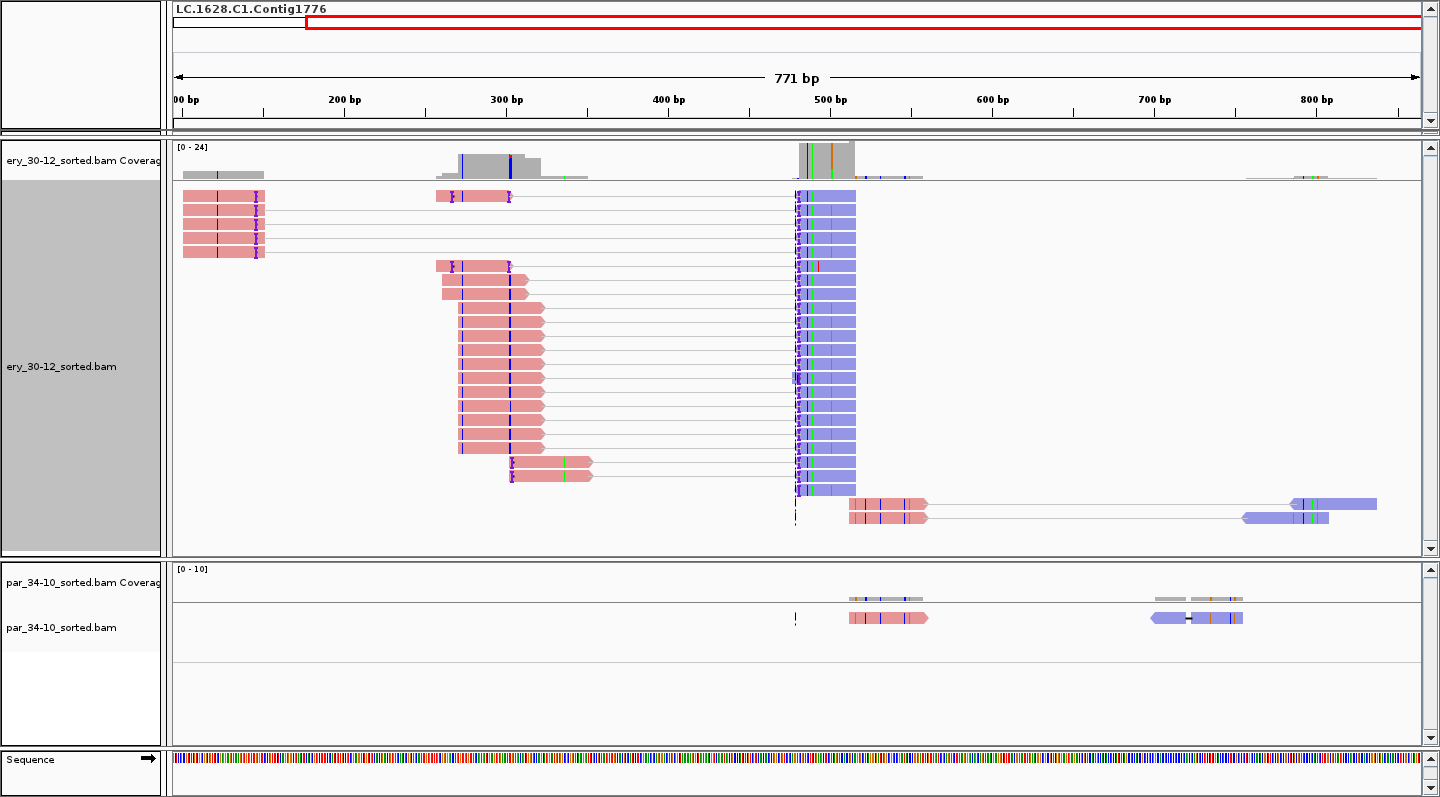
\includegraphics[width=\textwidth]{igv_LC_1628_C1_Contig1776_standRAD}
\caption{Alignment of standard RAD read pairs to both sides of an SbfI restriction site. Read pairs are connected by a line. Forward mapping reads are pink, backward mapping reads are blue. The upper individual has 7 unique read pairs, i. e. with different paired-end reads.}
\label{LC.1628.C1.Contig1776_standRAD}
\end{figure}

\texttt{find\_linked\_RADtags.pl} collects all paired-end reads that are mates of single-end reads that mapped to a detected \gls{linked RAD tag site}. It prints reads upstream or downstream of that site to separate files for each detected reference contig. 

%% ---------------------------------------------------------------------------------------------
\FloatBarrier
\subsection{de novo assembly of PE reads}\label{ch:PE_read_assembly}
%% ---------------------------------------------------------------------------------------------

I attempted to use \href{http://www.vicbioinformatics.com/software.velvetoptimiser.shtml}{\texttt{VelvetOptimiser.pl}} to assemble the collected \gls{pe} reads into PE contigs \citep{Zerbino2008}. However, the programme fails to assemble three PE read contigs with low read coverage -- Contig1776\_downstream (see figure  \ref{LC.1628.C1.Contig1776_standRAD}), Contig4139\_upstream and LC03019A1F03.f1\_upstream -- despite my diligent attempts to provide the necessary settings \citep{Zerbino2010}.

\texttt{SSAKE} \citep{Warren2007} is a simpler but also less heuristic and more tunable assembly programme than \texttt{Velvet}. It does not take base quality scores into account and takes only multi-fasta files as input. It searches for \emph{perfect} \gls{kmer} matches between reads. i. e. does not allow for sequencing error or \glspl{snp}.

\begin{cmd}
\captionsetup{type=cmd} % this is necessary for the hyperlink to work, see manual for caption package, 6.5 about hyperref
\begin{Verbatim}[fontsize=\scriptsize, formatcom=\color{darkgray}]

for i in ../*fq; do awk '(NR-1)%4==0 || (NR-2)%4==0' $i | sed 's/^@/>/' > `basename $i .fq`.fa; done
\end{Verbatim}
\caption[ fastq files into multi-fasta files]{Command line that turns fastq files into multi-fasta files. It takes all fastq files in the parent directory, extracts the header and sequence part (while skipping the quality string), replaces the "@" at the beginning of the fastq headers with a required ">" sign and writes the stream to a new file with the same base name.}
\label{fastq_to_fasta}
\end{cmd}

\texttt{SSAKE} by default does not allow setting a minimum overlap (\texttt{-m}) of less than 16 \gls{bp}. This could be too stringent for some of the low coverage PE contigs that I want to assemble. I, therefore, modified \texttt{SSAKE} to allow a minimum overlap of as small as 10 bp. When calling \texttt{SSAKE} with 
\begin{description}
\item[\texttt{-w 1}] Minimum depth of coverage allowed for contigs
\item[\texttt{-o 1}] Minimum number of reads needed to call a base during an extension
\end{description}
\dots ~on the "Contig1776\_downstream" reads for PE assembly (just two overlapping reads, see fig. \ref{LC.1628.C1.Contig1776_standRAD}), it is able to assemble a full length contig of 81 bp.

Any non-genomic sequence, i. e. adapter sequence, in the reads should interfere with de novo assembly. The Perl script \texttt{TagCle} by Kang-Wook Kim (Sheffield University) detects overlap between paired reads by Smith-Waterman local alignment and clips off read segments downstream of the end of the local alignment, i. e. generally adapter sequence. So this script can also detect a \emph{single} adapter (or barcode) base at the end of a read. I used command \ref{tagcle_run} to remove adapter sequences from the reads.

\begin{cmd}
\captionsetup{type=cmd} % this is necessary for the hyperlink to work, see manual for caption package, 6.5 about hyperref
\begin{Verbatim}[fontsize=\scriptsize, formatcom=\color{darkgray}]

$ for i in ../input/*fq_1; 
do (j=`echo $i | sed 's/1$/2/'`; TagCle_0.70.pl -me -i1 $i -i2 $j > `basename $i .fq_1`.log ) & 
done
\end{Verbatim}
\caption{The command line that I used in order to run Kang-Wook's script \texttt{TagCle} on all 154 pairs of input files in parallel. The \texttt{-me} switch turns off any direct search for adapter sequences.}
\label{tagcle_run}
\end{cmd}

\texttt{TagCle} clipped 159 SE and 216 PE reads of a total of 1,584,732 reads (0.02\%). It did not discard any sequence.

All de novo assemblers require optimisation of \gls{kmer} length, which is mainly what \texttt{VelvetOptimiser.pl} does with \texttt{Velvet}. So I wrote a script called \texttt{SSAKEoptimiser.pl} which iterates through \gls{kmer} lengths of 11 to 33 and keeps the assembly which produces the longest contig. This script exists in several parallelised versions (using different parallelisation modules) that parallelise not only over input files but also over iterations through \gls{kmer} lengths. This full parallelisation greatly speeds up execution on a multi-core machine (figure \ref{runtimes}).

\begin{figure}
\centering
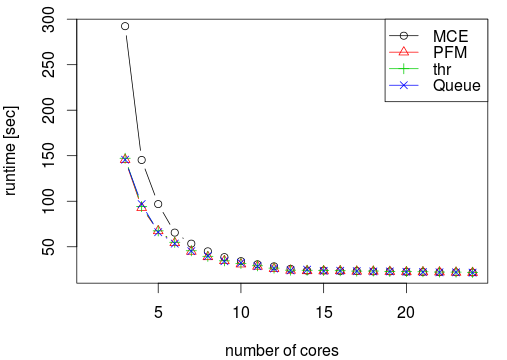
\includegraphics[width=.9\textwidth]{Parallel_Module_Comp}
\caption{The run times of the four parallelised versions of the \texttt{SSAKEoptimiser} script on 11 input files.}
\label{runtimes}
\end{figure}



\texttt{SSAKE} generally assembles many contigs for a region. In some cases this is due to different SE RADtags mapping to the same position in the \textit{Schistocerca} transcriptome. In other cases, this is clearly due to insufficient merging of contigs by \texttt{SSAKE} due to low coverage and SNPs (fig. \ref{contig_alignment})

\begin{figure}
\centering
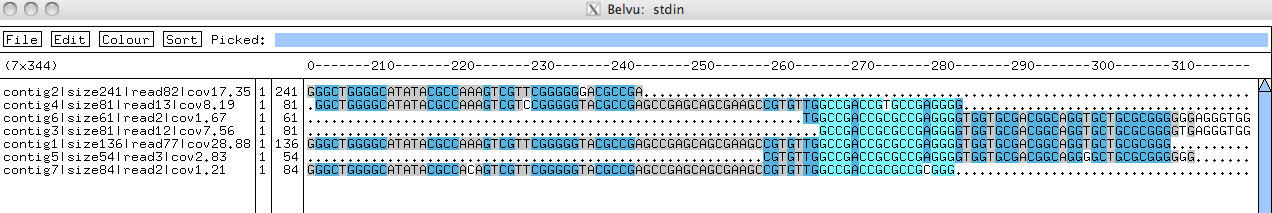
\includegraphics[width=\textwidth]{contig_alignment}
\caption{Multiple sequence alignment of \texttt{SSAKE} contigs assembled from reads collected from the downstream side of the RADtag site in the \textit{Schistocerca} reference contig "LC.1628.C1.Contig1776". The aligment view was created with the command: \texttt{muscle -in *LC.1628.C1.Contig1776\_downstream*contigs -msf | belvu -}~. The 7 contigs can clearly be merged into one big contig if allowing for a few SNP's.}
\label{contig_alignment}
\end{figure}

That's why I created multiple alignments of \texttt{SSAKE} contigs with \texttt{Muscle} \citep{Edgar2004} from each assembly in order to manually merge them in the alignment editor of \texttt{MEGA} \citep{Tamura2013}.


%% ---------------------------------------------------------------------------------------------
\FloatBarrier
\subsection{picking the right \texttt{SSAKE} contigs}\label{ch:picking_right_contig}
%% ---------------------------------------------------------------------------------------------

Since the \texttt{SSAKEoptimiser} output generally contains several \glspl{contig} of similar length and with similar read counts, it is difficult to pick those contigs upstream and downstream that genuinely belong together, i. e. come from the same locus. It is by no means always the longest \gls{contig} assembled that aligns significantly to the \textit{Schistocerca} reference\footnote{visual inspection of a pairwise alignment}.

For each PE read assembly, I determined the length of the longest contig assembled, the total number of contigs assembled as well as the number of contigs with length $>100$, $>200$ and $>300$ \gls{bp}.

An important piece of information for picking the right \texttt{SSAKE} contigs would be a significant \texttt{blast} hit against their putative \textit{Schistocerca} reference contig. So I extracted all 64 \textit{Schistocerca} reference contig sequences\footnote{also called \emph{unigenes}} from the \textit{Schistocerca} reference file with \texttt{samtools faidx} (see command \ref{samtools_faidx}).

\begin{cmd}
\captionsetup{type=cmd}
\begin{Verbatim}[fontsize=\scriptsize, formatcom=\color{darkgray}]
for i in `cat reference_contig_names_with_up-downstream_contig`; \
do samtools faidx LC_unique.seq  $i > $i.fa; \
done
\end{Verbatim}
\caption{\small Example of a command line that extracts fasta sequences from an indexed multi-fasta file using a file listing fasta headers.}
\label{samtools_faidx}
\end{cmd}

With my script \texttt{blast2seq.pl} -- calling \texttt{NCBI blastn 2.2.28+} \citep{Camacho2009} -- I then blasted all 128 relevant \texttt{SSAKE} contigs files against their putative \textit{Schistocerca} reference contig sequence and recorded the number of blast hits as well as the fasta headers of the 10 best hitting \texttt{SSAKE} contigs together with their \gls{e-value} (\href{http://blast.ncbi.nlm.nih.gov/Blast.cgi?CMD=Web&PAGE_TYPE=BlastDocs&DOC_TYPE=FAQ#expect}{further explanation}) in a \textsf{.SSAKE\_contig\_stats} file. I only recorded \texttt{blastn} hits with an \gls{e-value} of less than $10^{-10}$. I then used this table as a guide for picking and possibly merging \texttt{SSAKE} contigs in \texttt{MEGA}. I used command lines similar to \ref{blastn}, in order to find overlapping \texttt{SSAKE} contigs that haven't been merged by \texttt{SSAKE}.

\begin{cmd}
\captionsetup{type=cmd}
\begin{Verbatim}[fontsize=\scriptsize, formatcom=\color{darkgray}]
blastn -query *LC03012A1D06.f1_downstream.fa.ssake*.contigs \
-subject *LC03012A1D06.f1_downstream.fa.ssake*.contigs -task blastn \
-evalue 1e-10 -outfmt 6 | awk '$1 != $2' | sort -k3 -nk11 | awk 'NR%2' | less -S
\end{Verbatim}
\caption{\small This command line example is a very quick way to find out which sequences in a multi fasta file are similar to each other. It prints out hits of an all by all \texttt{blastn} of the sequences in a file. Note that query and subject get the same file. The first \texttt{awk} command removes hits against itself, the sort part brings reciprocal hits together and the second \texttt{awk} command keeps only one line for each pair of matching sequences.}
\label{blastn}
\end{cmd}

After picking and potentially merging \texttt{SSAKE} contigs, I aligned upstream and reverse complemented downstream\footnote{with respect to the restriction site} contigs against their putative \textit{Schistocerca} reference contig (if possible, i. e. significant blast hit) and filled the gap between them with N's. I thus created a new \emph{PE contig pair} consensus sequence for each \textit{Schistocerca} reference contig from upstream and downstream \texttt{SSAKE} contig sequences. 

%% ---------------------------------------------------------------------------------------------
\FloatBarrier
\subsection{Backmapping}\label{ch:Backmapping}
%% ---------------------------------------------------------------------------------------------

\subsubsection{Including SE RAD tag sequences into the new reference}

Before backmapping of all reads against the newly created PE contig pair reference, I wanted to include the SE \gls{RAD tag} sequences into the PE contig pair consensus sequences. For the determination of the consensus single-end sequences I obviously only want to use reads whose mate was used for the assembly of the \texttt{SSAKE} PE-contig that I finally picked (see section \ref{ch:picking_right_contig}). That's because \texttt{find\_linked\_Radtags.pl} had printed out all paired reads that mapped to a detected linked RADtags site in the \textit{Schistocerca} reference, but after the \texttt{SSAKE} assembly I mostly only picked PE-contigs that got a \texttt{blast} hit to their \textit{Schistocerca} reference contig. Other \texttt{SSAKE} contigs are much more likely to derive from similar but non-homologous loci to the \textit{Schistcerca} reference contig. I used command \ref{blast_mapping} in order to extract the fastq headers from those paired-end reads that get a blast hit to their inferred PE contig.

\begin{cmd}
\captionsetup{type=cmd}
\begin{Verbatim}[fontsize=\scriptsize, formatcom=\color{darkgray}]
for i in *fq_2; \
do awk '(NR-2)%4==0 || (NR-1)%4==0' $i | sed 's/@/>/' | sed 's/_pp//' | \
blastn -subject `basename $i .fq_2`_consensus.fas -evalue 1e-10 -outfmt 6 | \
cut -f1 | sed 's/2$/1/' > `basename $i .fq_2`_blast_mapped.ids; \
done
\end{Verbatim}
\caption{\small Using \texttt{blastn} to find PE reads that map to the inferred PE contig (see section \vref{ch:picking_right_contig}). The \texttt{for} loop iterates over all 40 PE read files. The first part of the loop converts fastq to fasta format. The second line feeds that into \texttt{blastn} (using megablast by default) and uses the corresponding PE contig (from section \ref{ch:picking_right_contig}) as subject. The third line takes the first column with the query headers from the blast output table and writes it to an output file.
}
\label{blast_mapping} 
\end{cmd}

I can then use these \texttt{*.ids} files, containing headers of the required SE sequences, as pattern files for a \texttt{grep} filter of the SE read files that \texttt{find\_linked\_RADtags.pl} has put out (see command \ref{grep_filter}).

\begin{cmd}
\captionsetup{type=cmd}
\begin{Verbatim}[fontsize=\scriptsize, formatcom=\color{darkgray}]
for i in *ids; \
do grep -A1 -f $i ../all_Big_Data_`basename $i _blast_mapped.ids`.fq_1 | \
egrep -v "\-\-" | sed 's/@/>/' > `basename $i .ids`_SE.fas; \
done
\end{Verbatim}
\caption{\small Using the header files created by the previous command (\ref{blast_mapping}) to extract corresponding SE reads from \texttt{find\_linked\_RADtags.pl} SE read files.}
\label{grep_filter}
\end{cmd}

I then created multiple sequences alignments with \texttt{muscle} in \texttt{.msf} format, which I could then use for the \texttt{consambig} programme from the \href{http://emboss.sourceforge.net/apps/release/6.6/emboss/apps/consambig.html}{\texttt{emboss}} package in order to create SE \gls{RAD tag} consensus sequences. I included these sequences into the 20 PE contig pair consensus sequences manually in \texttt{MEGA}. I used \texttt{stampy} to align all standard SbfI RAD reads from all 36 individuals against this new set of reference sequences.

\subsubsection{Targeted alignment and clean up of mapping result}

Figure \ref{stampy_par_34-10_vs_primer3ready_igv} shows an example of alignment of this \texttt{stampy} mapping. There are many low quality mappings which are very likely wrong (e. g. SE reads mapped to PE contig without SbfI site). However, here I have been using reads derived from a much larger source than is represented in the small reference of 20 \glspl{linked RAD tag site}. Therefore, \texttt{stampy} finds unambiguous mapping locations\footnote{indicated by a mapping quality >3} for reads that have an \gls{edit distance} of 17 to the reference sequence. \texttt{stampy} does not have an option for maximum allowed distance to the reference.

\begin{figure}
\centering
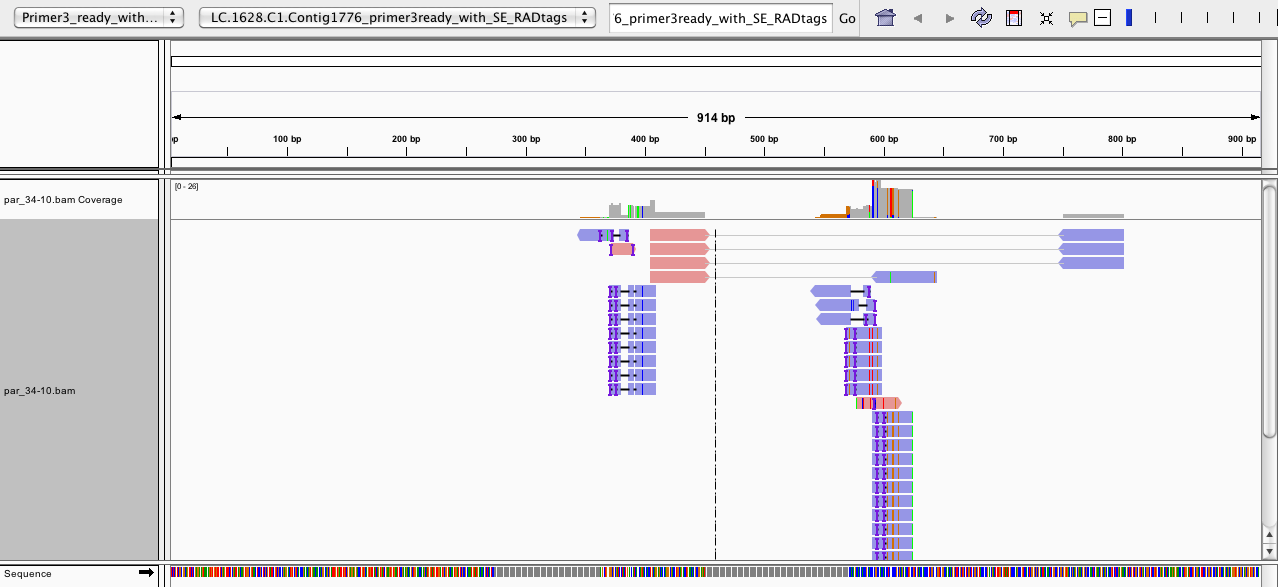
\includegraphics[width=\textwidth]{stampy_par_34-10_vs_primer3ready_igv}
\caption{Example read alignment of all standard RAD reads of individual par\_34-10 against one detected \gls{linked RAD tag site} sequence.}
\label{stampy_par_34-10_vs_primer3ready_igv}
\end{figure}

\cite{Kosugi2013} have developed a few Perl scripts that deal with the problem of false positive alignments especially when doing a so-called \emph{targeted alignment}\footnote{when the reference sequence is much smaller than the source of the reads to be mapped} by removing reads that map with too high a number of mismatches. They show that filtering by mapping quality score is rather ineffective when trying to improve a targeted alignment. 

\texttt{Coval-refine} by default removes all reads with more than 2 \glspl{indel}, 1 indel and 1 soft-clipped end and 2 soft-clipped ends. I have set the maximum proportion of mismatches to 0.1. The single-end reads are 46 base pairs long and are allowed to have up to 5 mismatches. The 51 base pair long paired-end reads are also allowed up to 5 mismatches.

\begin{figure}
\centering
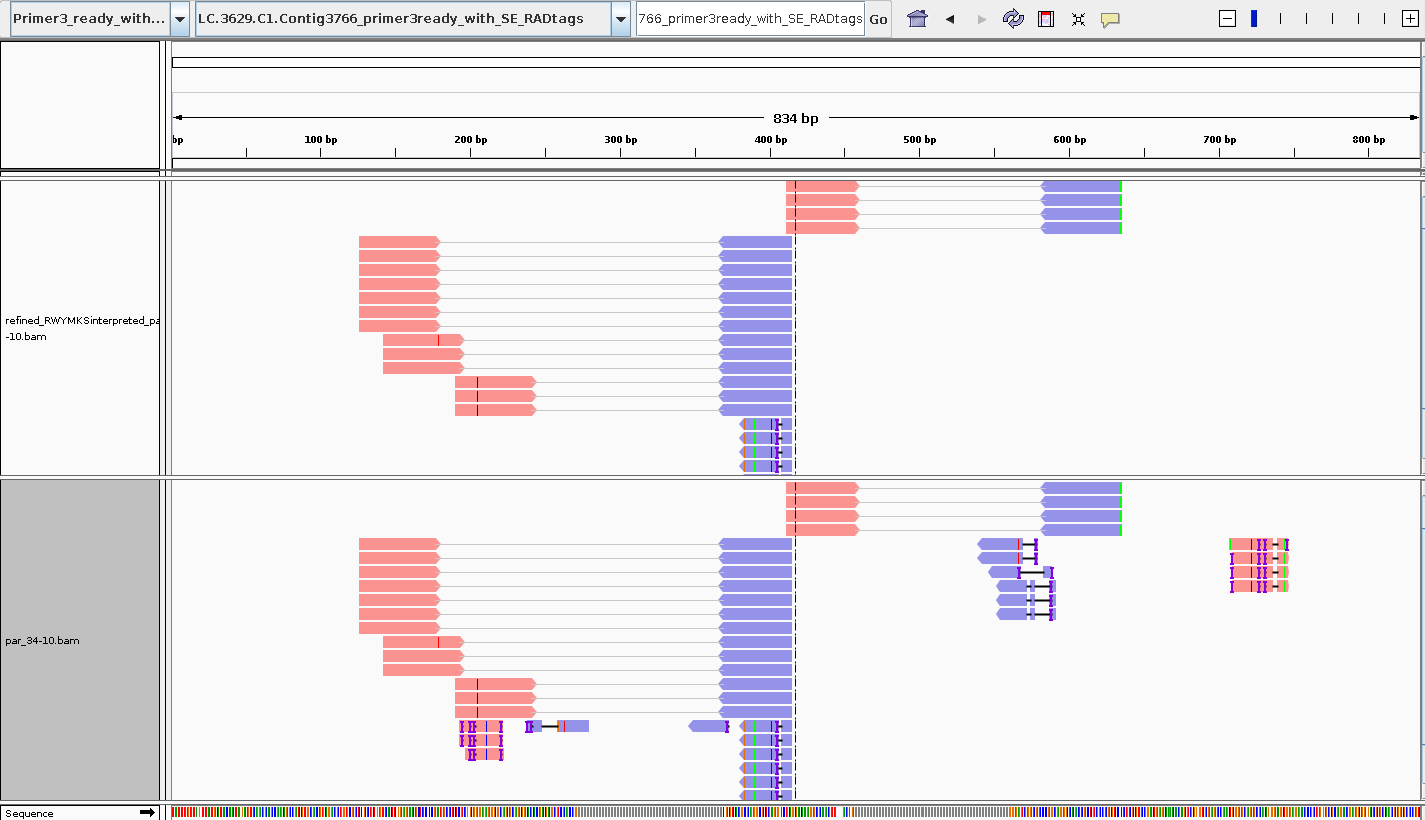
\includegraphics[width=\textwidth]{stampy_par_34-10_vs_primer3ready_after_coval-refine_igv}
\caption{Read alignment of all standard RAD reads of individual par\_34-10 against one detected linked RADtags sequence in the primer3ready\_with\_RADtags reference. Upper track after \texttt{coval-refine} filtering. Lower track is without \texttt{coval-refine} filtering for comparison.}
\label{coval-refine}
\end{figure}

Figure \ref{coval-refine} shows the mapping result after \texttt{coval-refine} treatment for one individual and one reference sequence.

By default, \texttt{coval-refine} counts ambiguous positions in the reference as mismatches. I changed \texttt{coval-refine-sam.pl} to take correct account of the dual ambiguity codes RWYMKS. I also made it count \glspl{indel} like two mismatches.

%% ---------------------------------------------------
\section{Estimating divergence time of the two subspecies}
%% ---------------------------------------------------

\begin{itemize}
\item work off questions
\item leave details including command lines for suppl. material
\item template amount estimation with fluorometer before and after PCR, qPCR
\item how much heterozygosity within populations, after long distance dispersal
\item leap-frog dispersal
\item Lunt, Cooper, Cpn1, mitochondria
\item ABS, simCoal
\item long dispersal tail --> potential for contact between distal populations
\item test gene flow <-> no gene flow model
\item filtering paralogs in highly repetitive genomes
\item large genome size $+$ genome size variation
\item clustering algorithms: DNAclust, CD-Hit, afcluster, ustacks, starcode, UNEAK
\end{itemize}


\section{Results}

\section{Interpretation of Results}



% ********************************************************
And now I begin my third chapter here \dots

\cite{Baird2008} were the first to publish about RAD. \SI{12,3}{\micro\metre}

Fig.~\vref{fragments-mapped-per-ind} shows the number of \glspl{fragment} mapped per individual.
I am trying to find \glspl{snp} among individuals of the sample.
% ********************************************************







\subsection{First subsection in the first section}
\dots and some more 

\subsection{Second subsection in the first section}
\dots and some more \dots

\subsubsection{First subsub section in the second subsection}
\dots and some more in the first subsub section otherwise it all looks the same
doesn't it? well we can add some text to it \dots

\subsection{Third subsection in the first section}
\dots and some more \dots

\subsubsection{First subsub section in the third subsection}
\dots and some more in the first subsub section otherwise it all looks the same
doesn't it? well we can add some text to it and some more and some more and
some more and some more and some more and some more and some more \dots

\subsubsection{Second subsub section in the third subsection}
\dots and some more in the first subsub section otherwise it all looks the same
doesn't it? well we can add some text to it \dots

\section{Second section of the third chapter}
and here I write more \dots

\section{The layout of formal tables}
This section has been modified from ``Publication quality tables in \LaTeX*''
 by Simon Fear.

The layout of a table has been established over centuries of experience and 
should only be altered in extraordinary circumstances. 

When formatting a table, remember two simple guidelines at all times:

\begin{enumerate}
  \item Never, ever use vertical rules (lines).
  \item Never use double rules.
\end{enumerate}

These guidelines may seem extreme but I have
never found a good argument in favour of breaking them. For
example, if you feel that the information in the left half of
a table is so different from that on the right that it needs
to be separated by a vertical line, then you should use two
tables instead. Not everyone follows the second guideline:

There are three further guidelines worth mentioning here as they
are generally not known outside the circle of professional
typesetters and subeditors:

\begin{enumerate}\setcounter{enumi}{2}
  \item Put the units in the column heading (not in the body of
          the table).
  \item Always precede a decimal point by a digit; thus 0.1
      {\em not} just .1.
  \item Do not use `ditto' signs or any other such convention to
      repeat a previous value. In many circumstances a blank
      will serve just as well. If it won't, then repeat the value.
\end{enumerate}

A frequently seen mistake is to use `\textbackslash begin\{center\}' \dots `\textbackslash end\{center\}' inside a figure or table environment. This center environment can cause additional vertical space. If you want to avoid that just use `\textbackslash centering'


\begin{table}
\caption{A badly formatted table}
\centering
\label{table:bad_table}
\begin{tabular}{|l|c|c|c|c|}
\hline 
& \multicolumn{2}{c}{Species I} & \multicolumn{2}{c|}{Species II} \\ 
\hline
Dental measurement  & mean & SD  & mean & SD  \\ \hline 
\hline
I1MD & 6.23 & 0.91 & 5.2  & 0.7  \\
\hline 
I1LL & 7.48 & 0.56 & 8.7  & 0.71 \\
\hline 
I2MD & 3.99 & 0.63 & 4.22 & 0.54 \\
\hline 
I2LL & 6.81 & 0.02 & 6.66 & 0.01 \\
\hline 
CMD & 13.47 & 0.09 & 10.55 & 0.05 \\
\hline 
CBL & 11.88 & 0.05 & 13.11 & 0.04\\ 
\hline 
\end{tabular}
\end{table}

\begin{table}
\caption{A nice looking table}
\centering
\label{table:nice_table}
\begin{tabular}{l c c c c}
\hline 
\multirow{2}{*}{Dental measurement} & \multicolumn{2}{c}{Species I} & \multicolumn{2}{c}{Species II} \\ 
\cline{2-5}
  & mean & SD  & mean & SD  \\ 
\hline
I1MD & 6.23 & 0.91 & 5.2  & 0.7  \\

I1LL & 7.48 & 0.56 & 8.7  & 0.71 \\

I2MD & 3.99 & 0.63 & 4.22 & 0.54 \\

I2LL & 6.81 & 0.02 & 6.66 & 0.01 \\

CMD & 13.47 & 0.09 & 10.55 & 0.05 \\

CBL & 11.88 & 0.05 & 13.11 & 0.04\\ 
\hline 
\end{tabular}
\end{table}


\begin{table}
\caption{Even better looking table using booktabs}
\centering
\label{table:good_table}
\begin{tabular}{l c c c c}
\toprule
\multirow{2}{*}{Dental measurement} & \multicolumn{2}{c}{Species I} & \multicolumn{2}{c}{Species II} \\ 
\cmidrule{2-5}
  & mean & SD  & mean & SD  \\ 
\midrule
I1MD & 6.23 & 0.91 & 5.2  & 0.7  \\

I1LL & 7.48 & 0.56 & 8.7  & 0.71 \\

I2MD & 3.99 & 0.63 & 4.22 & 0.54 \\

I2LL & 6.81 & 0.02 & 6.66 & 0.01 \\

CMD & 13.47 & 0.09 & 10.55 & 0.05 \\

CBL & 11.88 & 0.05 & 13.11 & 0.04\\ 
\bottomrule
\end{tabular}
\end{table}

%----------------------------
% Bibliography
%----------------------------

\bibliographystyle{elsarticle-harv}
\bibliography{/Users/Claudius/Documents/MyLiterature/Literature}

\end{document}
